\documentclass[fleqn,usenatbib,useAMS]{mnras}

\usepackage{graphicx}
\usepackage{amsmath}
\usepackage{multicol}
\usepackage{bm}
\usepackage{pdflscape}

\usepackage[T1]{fontenc}
\usepackage{ae,aecompl}

\usepackage{newtxtext,newtxmath}

\title[Relativistic disc lines]{Relativistic lines from thick discs in different spacetimes}

% after talking to Fergus, he preferred me being the first author
% thank you Fergus <3 
\author[W. Tarnopolska, et al.]{W. Tarnopolska$^{1}$\thanks{Contact e-mail: \href{mailto:wiktoria.tarnopolska@bristol.ac.uk}{wiktoria.tarnopolska@bristol.ac.uk}}, F. Baker$^{1}$, and A. J. Young$^{1}$ \\
$^{1}$HH Wills Physics Laboratory, Tyndall Avenue, Bristol BS8 1TL}

\date{Last updated \today}

\pubyear{2024}

\begin{document}
\label{firstpage}
\pagerange{\pageref{firstpage}--\pageref{lastpage}}
\maketitle

% cut down on gradus info -- say what it can do, briefly what we implemented

% elaborate on taylor&reynolds shortcomings -- fix the claim / reach out and request the code

% put the code today,, link the paper

% table models code

\begin{abstract}
This work explores the physics and astrophysics of black holes, focusing on the study of iron lines in the emission spectra of accretion flows close to the central black hole. Iron lines are important probes for studying the strong gravitational fields generated by black holes, enabling tests of general relativity in the strong field regime. 

So far, models focus on the thick discs in standard spacetimes, which can be extended to non-standard (Kerr--like) models. These models however, do not consider self--consistent illumination of the thick accretion disc by the corona, with particular drawbacks for geometries with multiple variable parameters and rely strongly on the approximation of the emissivity calculation using the power law, which compromises the importance of geometry in the interpretation of the emission lines. These models are typically costly to calculate and are strongly constrained by the number of variables and spacetime geometries. 

We aim to address these shortcomings using a novel iron line model was developed using the {\tt Gradus.jl} code, which allows for the self-consistent calculation of a metric with multiple deformation parameters in high resolution and with significantly improved calculation time.

The iron line model was tested by reproducing results from the literature, demonstrating that iron line profiles serve as an additional test of currently used numerical simulations. The model was then used to explore the impact of the Eddington ratio on the accretion disc, revealing that the influence of deformation parameters diminishes for non-spinning black holes and becomes more pronounced for spinning cases. 

\end{abstract}

\begin{keywords}
black hole physics -- accretion, accretion discs -- line: profiles
\end{keywords}

\section{Introduction}

% Test of physics + spacetime close to BH
Black holes are among the objects producing the most violent environments in our Universe. These exotic entities cause some of the most extreme physics observed, rightfully captivating the interest of the scientific community. The gravitational pull generated by black holes creates a strong gravity regime where the physics becomes much more interesting -- especially in the close vicinity to the horizon. 

Being the most efficient engines in the Universe \citep{rees1984black}, accretion onto a black hole is a cause of a variety of riveting curiosities in both active galactic nuclei and X-ray binaries \citep{taylor2018exploring}. Despite the complex astrophysics and some of our most fundamental physics failing in their vicinity, black holes remain fairly straightforward in their characteristics, as they can only hold information about three of their parameters -- mass $M$, angular momentum $J$, and charge $Q$. Although it is worth noting, that in astrophysical settings the charge will dissipate due to vacuum polarisation \citep{reynolds2003fluorescent}, it remains an interesting aspect in theoretical modelling. For this purpose, a black hole is completely described by its mass $M$ and spin $a = J/M$.

Therefore, black holes, being such fascinating objects, provide an exciting test of our understanding of physics, both extreme and fundamental. 

% BHs as tests of GR -- motivation
In particular, general relativity, despite behaving as predicted in most environments, exhibits interesting deviations in the strong field regime. Hence, black holes prove to be excellent probes for exploring this problem, enabling tests of general relativity within their strong gravitational fields.

% BHs iron lines importance -- motivation
The strong gravitational forces cause the iron lines in the black hole emission spectra to change in shape due to the Doppler effects and gravitational redshift \citep{fabian2000broad}. Iron lines are an important tool, allowing the study of the geometry and properties of an accretion flow close to the central black hole. 

There are two distinct approaches to modelling black holes iron line profiles. The first one utilises approximation of the emissivity calculation using the power law, where the intensity is proportional to a constant power of pseudo-cylindrical radius \citep{abdikamalov2020testing}, however, this approach compromises the importance of geometry in the interpretation of the emission lines.

It has been proven that the black hole geometry including an irradiating source of radiation strongly influences the iron line shape \citep{dauser2016relativistic}. Such a model involves placing a corona above the black hole, which illuminates the accretion disc, and the emissivity profile is then self-consistently calculated. 

% motivation
This work was motivated directly by the intrinsic relation between the behaviour of iron lines and relativistic effects. Models proposed so far have their limitations. Specifically, it has not been possible to model a metric with multiple deformation parameters self-consistently before. Using {\tt Gradus.jl} it was possible to write a model that allows such calculation in high resolution and with significantly improved calculation time when compared to current works.

% % test of existing models
% Additionally, the iron line model was tested before this novel implementation, by reproducing results from the literature. This shows that iron line profiles serve an additional purpose, which is that of a test of currently used numerical simulations. 

\begin{figure*}
    \centering
    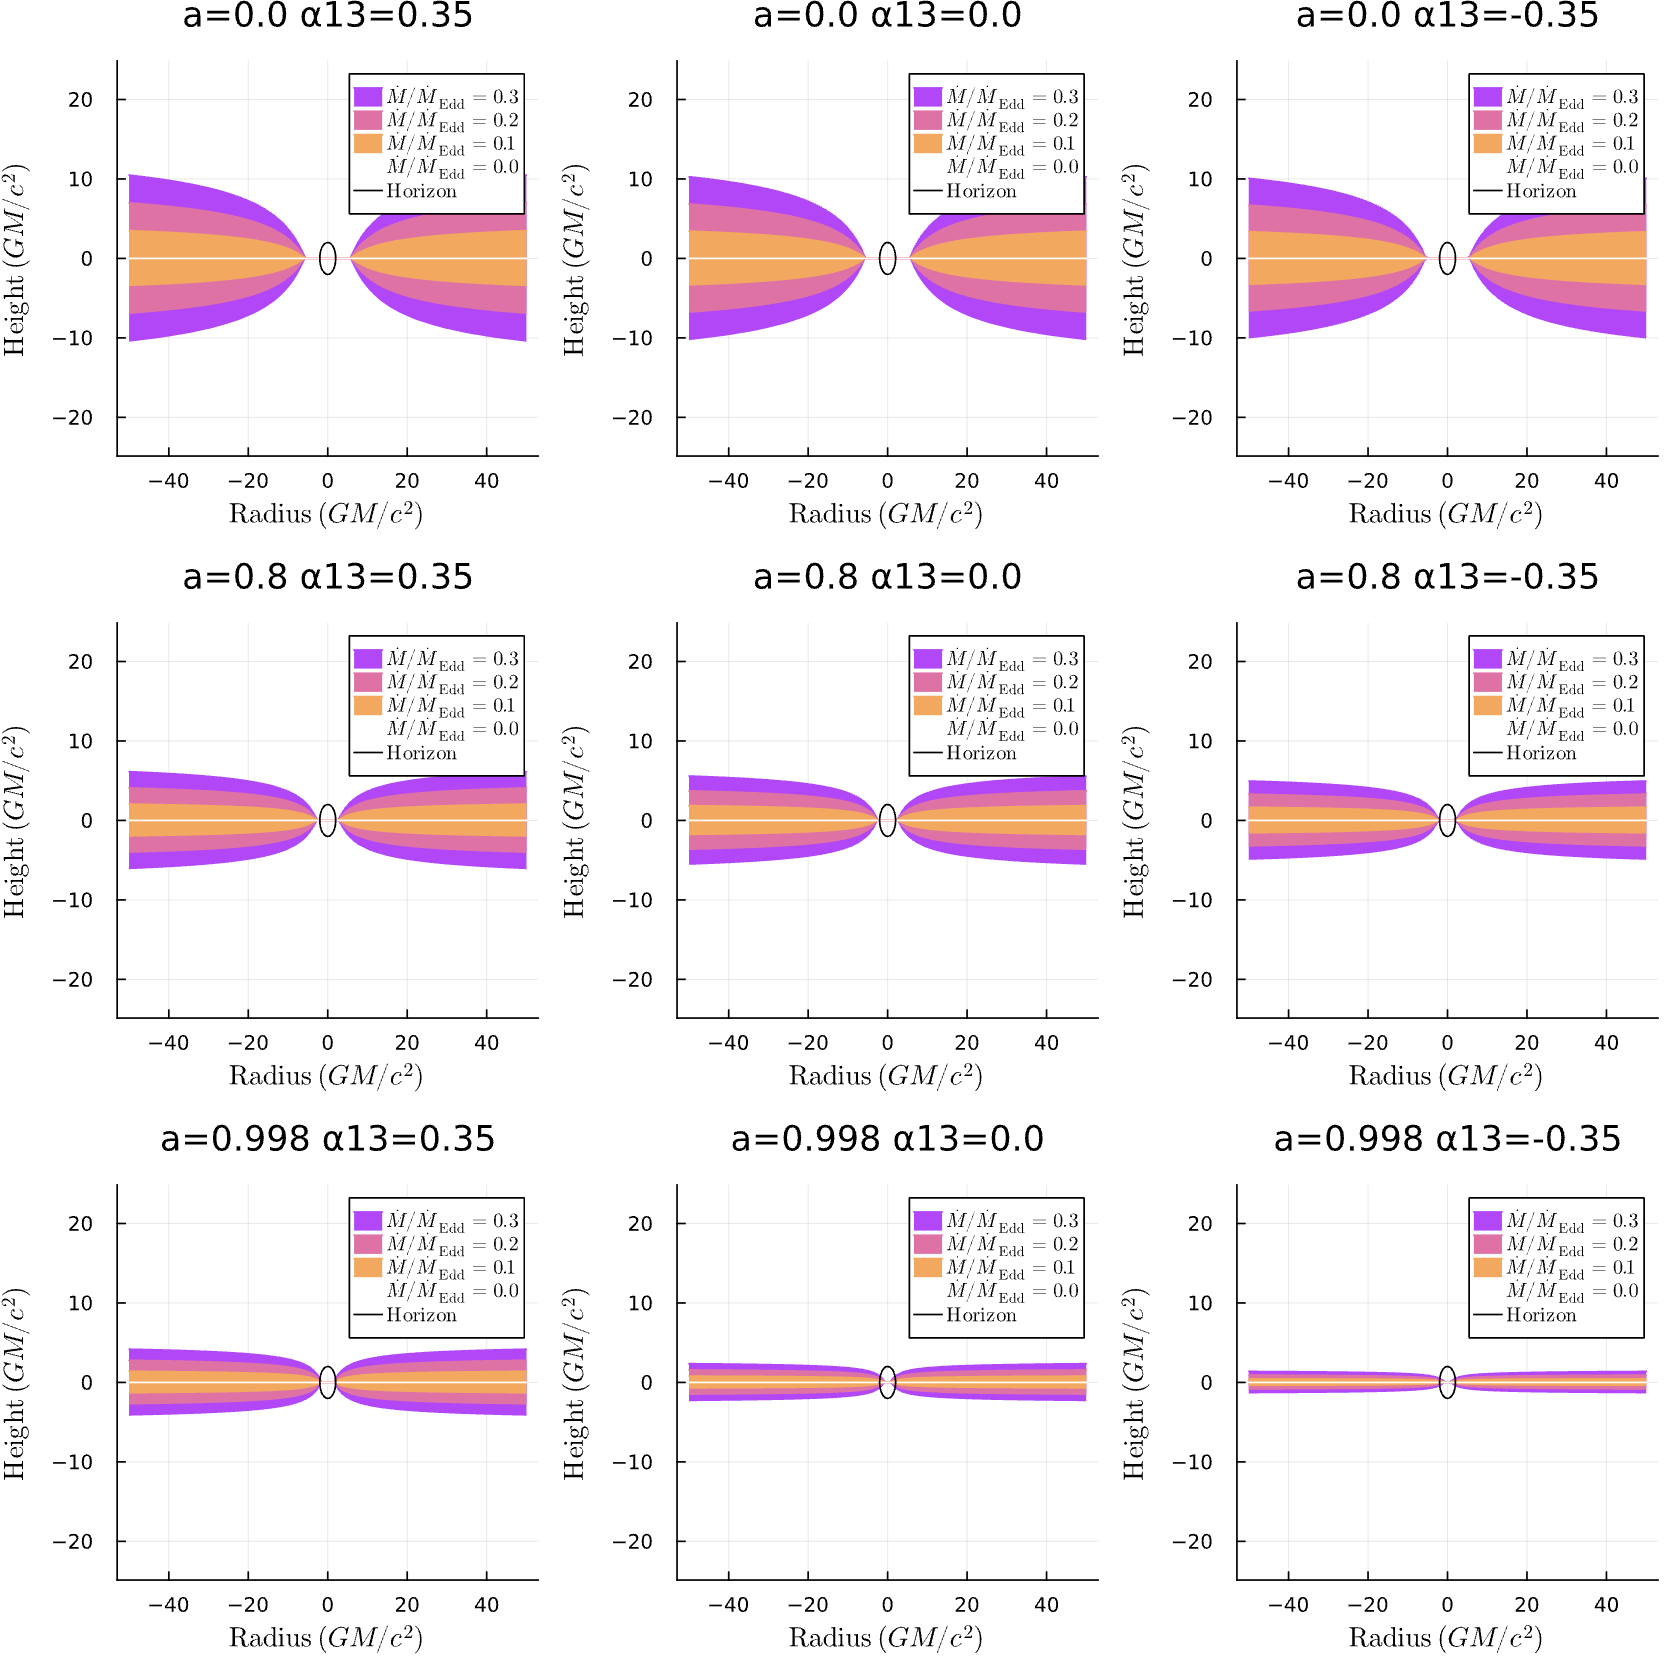
\includegraphics[width=0.98\linewidth]{figures/abdikamalov20.png}
    \caption{Profiles of black holes accretion discs for a non-rotating $a = 0$, rapidly rotating $a = 0.9$ and maximally rotating $a = 0.998$ case in the Johannsen metric with the deformation parameter $\alpha_{13} = -0.35, 0, 0.35$. Influence of $\alpha_{13}$ diminishes for $a = 0.0$ and becomes more pronounced for the spinning cases. Flattening of the disc can be observed for a maximally rotating black hole.}
    \label{eddingtonratio}
\end{figure*}

\section{Theory}
% --> impact of eddington ratio on the disc
The disc model implemented in this work is the classic \cite{shakura1973black} model which emulates a geometrically thin, optically thick disc with height scaling as
%
\begin{equation}
    H=\frac{3}{2\eta} \left[\frac{\dot{M}}{\dot{M}_\text{Edd}}\right]\left [1-\left(\frac{r_\text{ISCO}}{\rho}\right)^\frac{1}{2}\right]
    \label{height}
\end{equation}
%
where $\eta$ is the radiative efficiency, $r_\text{ISCO}$ the innermost stable circular orbit (ISCO) which also defines the inner edge of the disc, and $\rho = r \sin\theta$ is the pseudo-cylindrical radius dependent on $\theta = \frac{\pi}{2}$ which is the plane of the disc. 

$\frac{\dot{M}}{\dot{M}_\text{Edd}}$ represents the Eddington ratio, which is a scaled mass-accretion rate. The visualisation of the dependency of the disc shape on this value is depicted in Figure \ref{eddingtonratio} and was created directly using Equation \ref{height}. 
Notably, for a non-rotating case, the deformation parameter is not observed to impact the height of the accretion disc unless the spin is increased. The biggest influence of the deviation parameter occurs for a maximally rotating black hole and the higher the value the taller the disc becomes. However, as the black hole spins more rapidly, the disc becomes flatter, therefore decreasing the impact of the parameter across the different thicknesses.
Since both $r_{\text{ISCO}}$ and $\eta$ are functions dependent on the metric, the Eddington ratio can be treated as the disc thickness parameter \citep{abdikamalov2020testing}.

Following the logic presented in \cite{abdikamalov2020testing}, Figure \ref{eddingtonratio} represents a Johannsen metric with the only non-zero deformation parameter being $\alpha_{13}$ while all other parameters are set to zero for all values of spin.

Although this approach was implemented by \cite{abdikamalov2020testing} to maintain consistency with literature \citep{taylor2018exploring}, it is important to note that the actual relativistic scaled height will be different than the one derived from the Newtonian Shakura-Sunyaev model and the current one overestimates the effect associated with the Eddington ratio. 

% --> (emission) iron lines
The shape of the disc is intrinsically related to the relativistic effects and in turn to the shape of the spectrum observed from a black hole. The most prominent line in the spectrum is the iron K$\alpha$ line in the X-ray band occurring at 6.4 -- 6.9 keV observed in the spectrum of many active galactic nuclei (AGNs), particularly Seyfert galaxies \cite{fabian2000broad}. The fluorescent K$\alpha$ emission line of cold iron occurs due to the process of X-ray reflection -- it is produced when one of the two K-shell electrons of iron in either atom or ion form is ejected in the process of photoelectric absorption of an X-ray \cite{fabian2000broad} and serve as an important tool in probing information about its structure, geometry and spin of the central compact object \cite{reynolds1999x}. As the K$\alpha$ iron line is very susceptible to relativistic effects, it enables their observational study, revolutionising modern astrophysics.

Broadening of the lines due to the black hole spin requires the iron line to be emitted from the inner regions of the disc \cite{laor2005line}. This effect was theoretically predicted \cite{stella1990measuring}, although initially lacking observational confirmation. It was the analysis of data from MCG--6-30-15 \cite{tanaka1995gravitationally} that confirmed that broadening of the initially narrow iron line does in fact require emission from regions in the close vicinity of the black hole.

% -> impact of GR 
% 	Relativistic effects (Doppler gravitational redshift)
% 	On shape of the iron lines

Effects of general relativity due to strong gravitational fields close to the black hole significantly distort this region. This includes effects such as the Doppler-broadening, gravitational, and transverse redshifts \cite{fabian1989x}, all affecting the iron line profile uniquely, dependent on inclination. However, the gravitational redshift always leads to a broadening of the lines. The characteristic two-horned shape of the line changes due to aberration, time dilation, and blueshift, all dependent on the inclination of the observer and size of the relevant area of the disc -- this causes the discrepancy between the sizes of the two peaks. The spectrum emitted by the black hole will therefore get relativistically distorted before it reaches the observer \cite{dauser2016relativistic}. 

% --> photon index how it changes (ref Fanton)
Various parameters can impact the shape of emission line profiles as outlined in \cite{fanton1997detecting}. Example variations of the observer's inclination angle $\theta$, accretion disc emitting zone (space spanned between $r_{\text{in}}$ and $r_{\text{out}}$) and the emissivity index ($p$) following the broken power law
%
\begin{equation}
    I_{e} \approx r^{-p}
    \label{intensity}
\end{equation}
%
for two black holes with different values of spin, $a$ are shown in Figure \ref{fanton}. In this comparison, the value of the emissivity index $p = 2$ was implemented unless otherwise stated, as per example with the varied index itself using the {\tt Shakura-Sunyaev} disc model.

Observationally, decomposing the reflection spectrum of the NLS1 galaxy 1H 0707-495 \cite{wilkins2011determination} showed that the emissivity profile follows a trend of a twice-broken power law with index over 7, falling steep in a line over the the inner disc region, flattening over the intermediate region and then acutely falling over the outer part of the disc, which is the expected form of the irradiation profile in the vicinity of a black hole curving the space-time and illuminated by a corona \cite{suebsuwong2006gravitational}, \cite{wilkins2015driving}.

% consult -- red wing --> higher energies, lower frequency shift
Commonly, the profiles are asymmetric, and, as mentioned before, double-peaked, although that can change due to relativistic effects at play. Two distinctive features are the two peaks, often referred to as the \textit{blue wing} and the \textit{red wing}. The blue wing is shifted towards higher energies relative to energies on the rest of the line. Respectively, the red wing is shifted to lower energies relative to the rest of the line profile. In most cases, the higher peak is usually blueshifted, corresponding to higher frequency shifts \cite{fanton1997detecting}. 

\begin{figure}
    \centering
    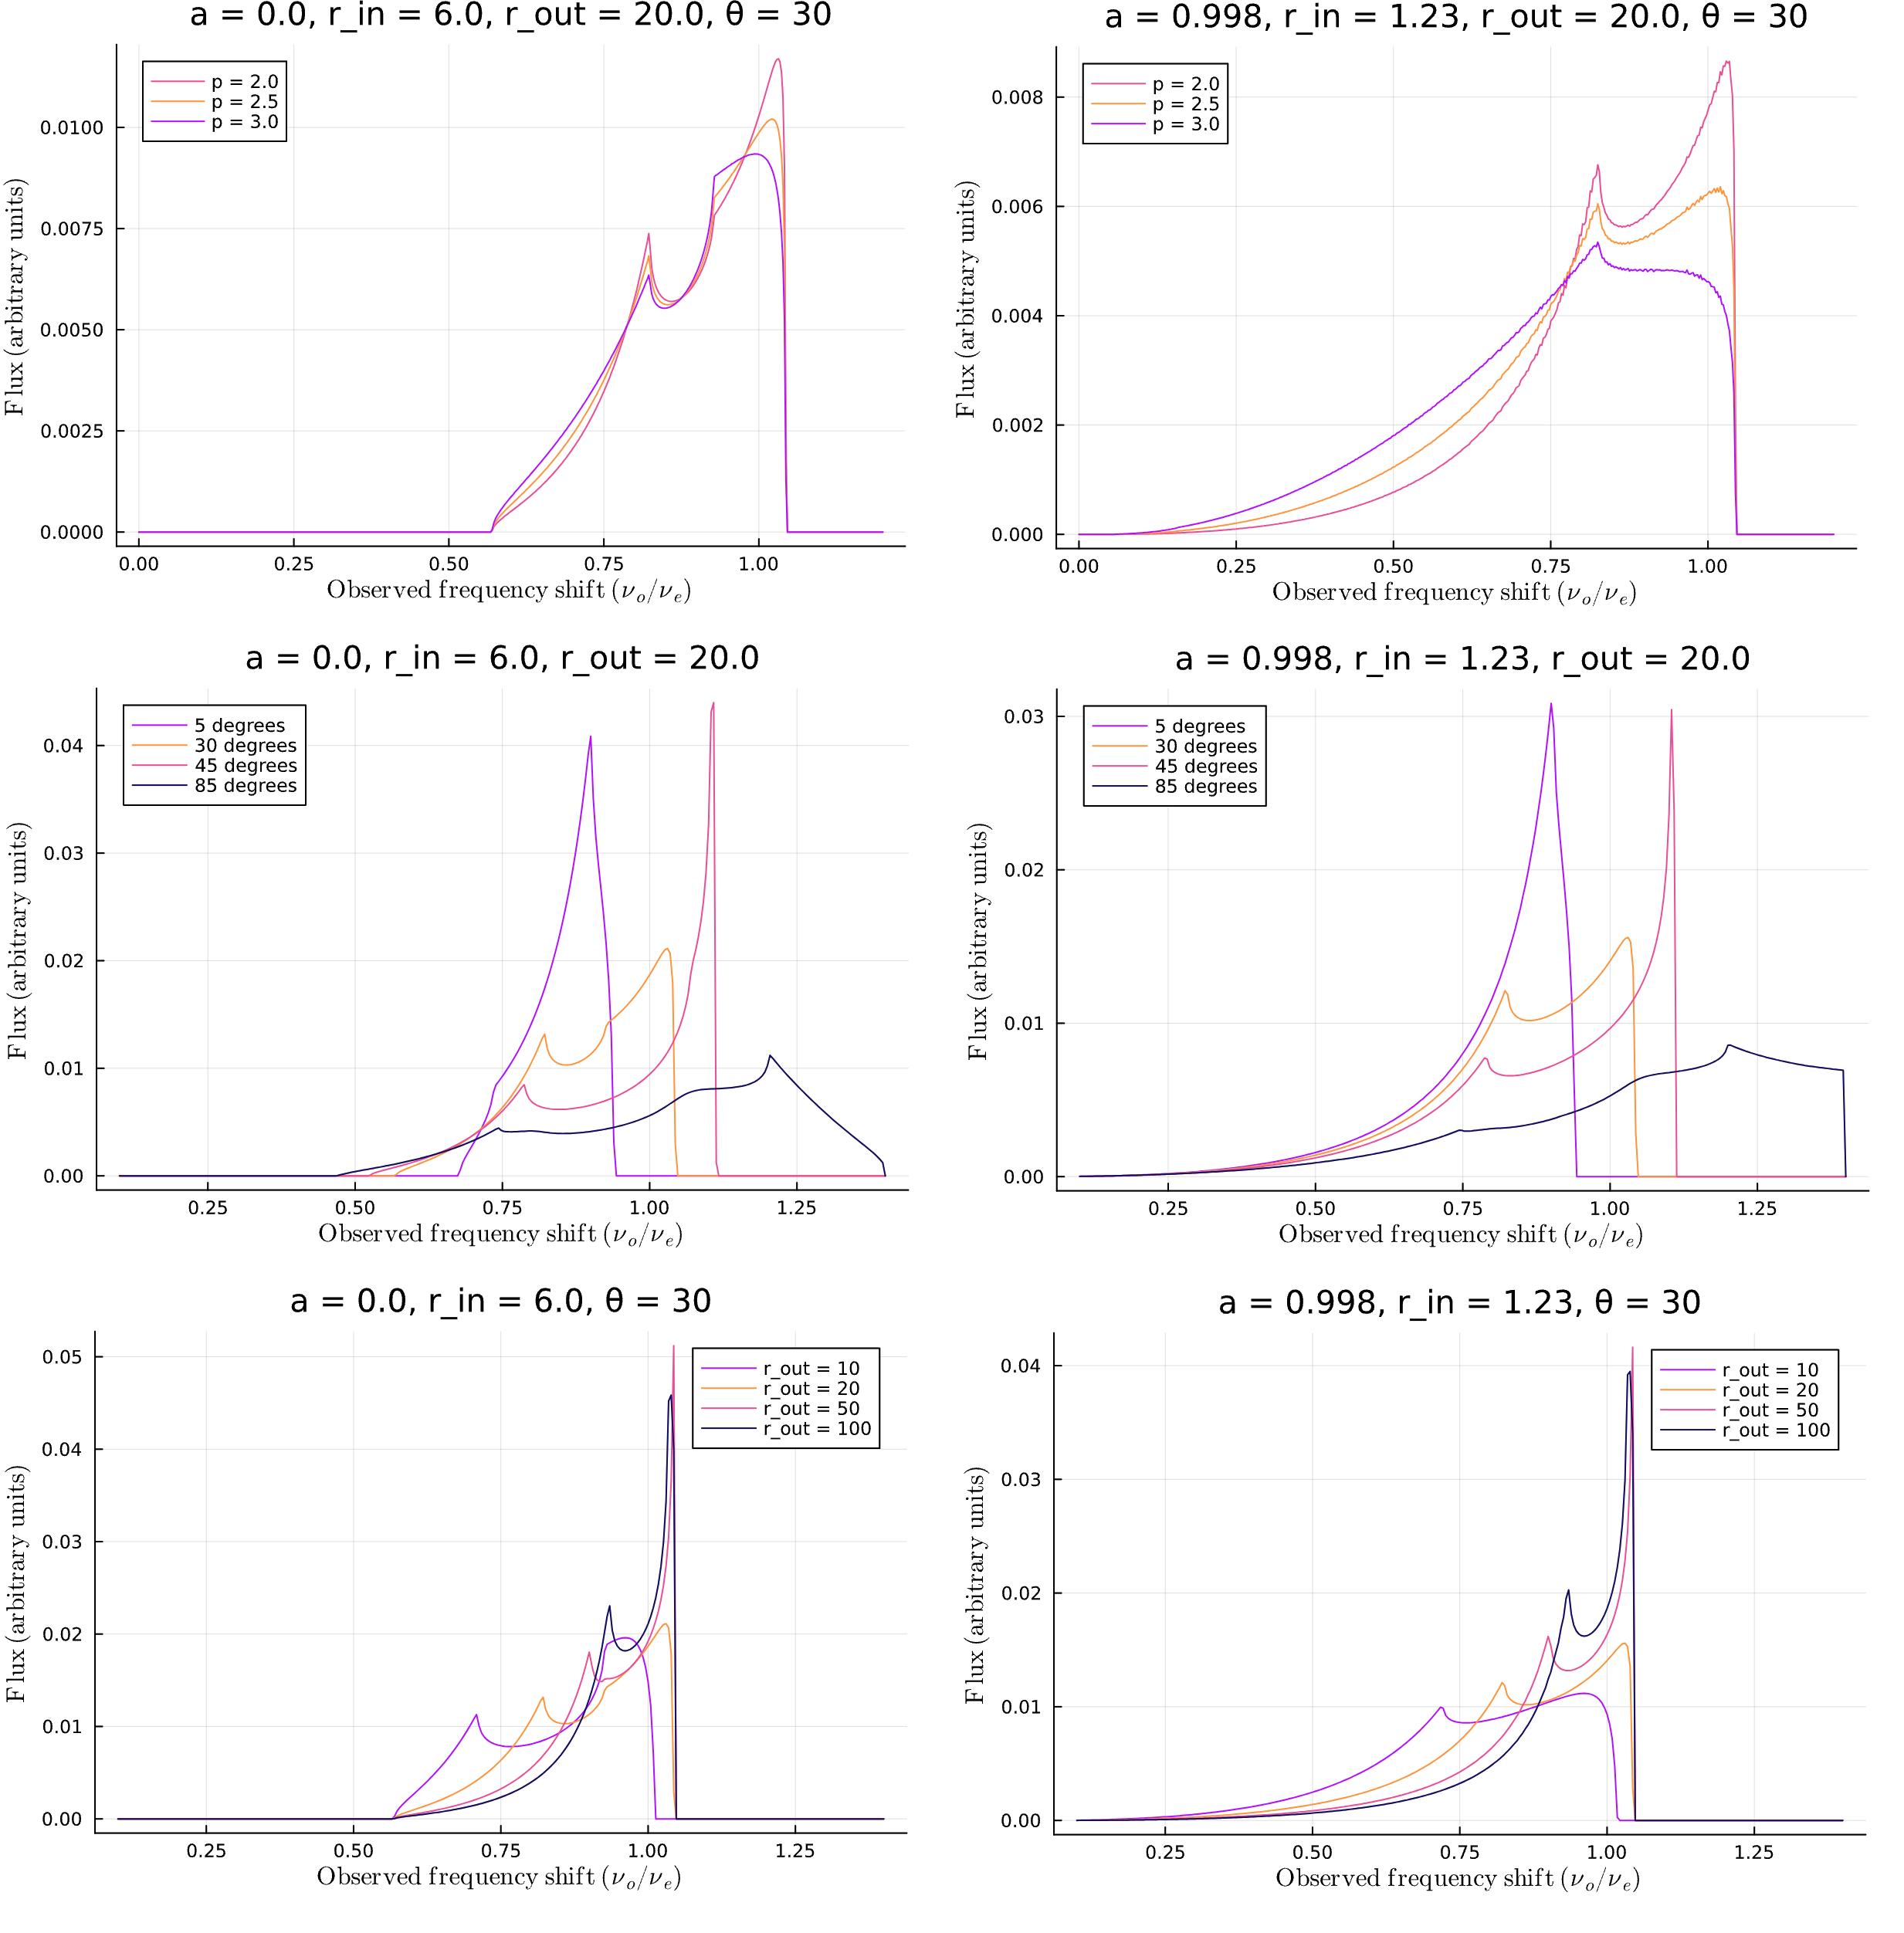
\includegraphics[width=0.98\linewidth]{figures/fanton.png}
    \caption{Iron line profiles of two black holes -- Schwarzschild non-rotating $a = 0$ (left column) and Kerr maximally rotating $a = 0.998$ (right). Effects of varying the photon index $p$ (first row), inclination angle (second row), and outer radius $r_{\text{out}}$ (third row) are shown. The inner radius was set to be 6.0 for the Swarzschild case and 1.23 for the Kerr case.}
    \label{fanton}
\end{figure}

This comparison shows that both increasing the inclination angle of the observer as well as the $a/M$ ratio results in the broadening of the iron line profiles.

% --> broken power law (emissivity)
X-ray spectrum is expected to be accurately approximated by the power law for energies up to about 100 keV \citep{brenneman2006constraining}. While \cite{fanton1997detecting} used the emissivity index $p = 2$, \cite{abdikamalov2020testing} chose $p = 3$. The other difference is that the former implements a power law as a function of the radius, while the latter replaces it with the pseudo-cylindrical radius $\rho$. This change is justified as it ensures a direct correspondence between every value of $\rho$ and every point on the disc due to its cylindrical symmetry. 

% --> self-consistent models (lamppost)
Self-consistent calculations involve inserting a corona into the black hole geometry. In this approach, the illumination pattern on the disc is calculated without approximating the surface intensity using the power law function. However, the presence of corona does give rise to a power law in the X-ray continuum illuminating the disc. Physically, the emissivity is the flux reflected off the disc, which is dependent on the flux of incident photons, which in turn is the projection of the intensity coming from the corona. However, the irradiation itself is calculated \textit{self-consistently} without the power-law approximation.

In order to properly account for this flux, a certain geometry needs to be chosen for the corona. Amongst one of the most well-established stands out the lamp post model. It describes the corona as an isotropic point source, located at a certain height above the disc plane on the black hole rotation axis. This model provides a good description for the primary source, although it is worth noting that the physical corona is most likely extended \citep{wilkins2015driving}. 

Emission of energetic particles from the corona irradiates the material in the accretion disc orbiting the central black hole \citep{george1991x} which is then reflected in the form of X-rays either through Compton scattering, photoelectric absorption, emission of fluorescent lines or bremsstrahlung \citep{ross2005comprehensive}.

The corona proves important in the broadening of the iron lines and allows for judgement of how the innermost parts of the disc contribute to the reflection spectra. A shortcoming of the power law approximation is that it does not show the expected steepness at the small radii, which is in turn automatically accounted for when performing the self-consistent calculations utilising the lamp post geometry \citep{dauser2016relativistic}. 

% --> Johannsen metric
Regarding the metric, \cite{abdikamalov2020testing} employ a metric proposed by Johannsen in 2013 \cite{johannsen2013regular}. Black holes are characterised completely by a Kerr metric dependent on mass $M$ and spin $a$. Multiple metrics including parameters describing deviation from this metric have been proposed. As argued by Johannsen, his proposed metric, expanded by four additional deformation parameters: $\alpha_{13}$, $\alpha_{22}$, $\alpha_{52}$ and $\epsilon_{3}$ offers a spacetime well-suited for tests of the no-hair theorem in the strong-field regime. Additionally, the deformation parameters need to satisfy the following conditions outlined by \cite{johannsen2013regular}:
%
\begin{equation}
    \alpha_{13} > - \frac{(M + \sqrt{M^2-a^2})^3}{M^3}
    \label{alpha13}
\end{equation}
%
\begin{equation}
    \alpha_{22} > - \frac{(M + \sqrt{M^2-a^2})^2}{M^2}
    \label{alpha22}
\end{equation}
%
\begin{equation}
    \alpha_{52} > - \frac{(M + \sqrt{M^2-a^2})^2}{M^2}
    \label{alpha52}
\end{equation}
%
\begin{equation}
    \epsilon_{3} > - \frac{(M + \sqrt{M^2-a^2})^3}{M^3}
    \label{epsilon3}
\end{equation}
%
% --> other metrics
Whilst the Kerr metric is one of the four black hole solutions of general relativity, the Johannsen metric generally is not a solution to the field equations of any specific theory of gravity. However, it can be mapped to known four-dimensional black hole solutions of modified theories of gravity for appropriate choices of the deviation functions \citep{johannsen2013regular}.
The other three solutions include Schwarzschild non-rotating, non-charged black hole, Kerr-Newman rotating and charged black hole, and Reissner-Nordstrom -- non-rotating black hole endowed with electric charge.

%clear objectives of the work

This work aimed to test the effects of general relativity in consistency with the literature, following the works of  \cite{abdikamalov2020testing} and \cite{taylor2018exploring} and building up to the novel implementation of a newly designed software to perform self-consistent simulations of the \cite{johannsen2013regular} metric for the first time. Whilst the aforementioned work of Abdikamalov models the Johannsen metric, it employs a power law to approximate the illumination pattern of the disc. This metric has not been modelled self-consistently before and this is the novelty of this work. Utilising {\tt Gradus.jl} -- a new photon ray tracing code by \cite{baker2022} it was possible to solve the Johannsen metric self-consistently while varying multiple parameters. Such an advancement has not been presented in the literature before. 


\section{Method} 

% --> overrun of code used
{\tt Gradus.jl} \cite{baker2022} is the software used throughout this work, providing accuracy, great resolution of the images and outstanding computation time. Unlike ordinary ray tracing, when accounting for relativistic ray tracing it is the nuance of the curvature of spacetime that needs to be considered and appropriately addressed. General relativity impacts the energetics of the system itself and therefore requires specific care in numerical modelling.

In the line model created for the purposes of this work, the main element is the calculate {\tt lineprofile} function which uses the {\tt Transfer function} method of calculating the profiles. The function allows specification of emitting region between ${\tt minr_{e}}$ and ${\tt maxr_{e}}$ which is essentially $r_{\text{in}}$ and $r_{\text{out}}$ of the disc. The function is capable of self-contained calculations of the ISCO, as well as accepting a given value. Resolution can also be specified, albeit at a cost of computation time if set too high, although to produce images with a good resolution the rendering time is still performing up to a satisfactory standard, especially when compared to other models available.


The spectrum is an argument defined as the power law from Equation \ref{emissivity}, noting the difference between the approximation and the power law present in the spectrum continuum for the self-consistent model. This one depends on the photon index $\Gamma$, as opposed to the emissivity index $p$. 

The disc is the aforementioned Shakura-Sunyaev \cite{shakura1973black} model, which is a function of the spacetime metric and the Eddington ratio.

There is an interesting problem to be mindful of when handling transfer functions at high inclination angles. When modelling iron line profiles at extremely high or low inclinations, the transfer functions calculations get complicated. In our case, this resulted in infinitely high spikes in the line spectra, particularly for high Eddington ratios. Further investigation of the problem rendered an interesting conclusion -- when the Eddington ratio increases and the disc expands, simultaneously becoming thicker, an observer viewing the black hole from a high inclination angle cannot see all of the disc clearly. Due to increased thickness, the disc starts obscuring itself. This was handled by offsetting its centre only minorly, which appeared to have solved the problem.

% --> transfer function vs binning method
The {\tt Transfer functions} method makes use of the Cunningham transfer functions \cite{cunningham1975effects} and is the default method in calculating the line profiles using {\tt Gradus.jl}. However, another method is also available, namely the binning method. 

The binning method operates by dividing the accretion disc and summing up contributions from each part. The disadvantage of the binning method lies in its resolution as it assumes the photon flux across every part to be uniform even if it is not the case. Using an analogy of a grid being placed over the disc, the binning method is assuming the flux is uniform across the whole cell. Moreover, particularly at the outer edge of the accretion disc, the method performs the calculation as if the whole cell was occupied by part of the disc, which is not very accurate and might lead to overcounting the incident photons.


\begin{figure*}
    \centering
    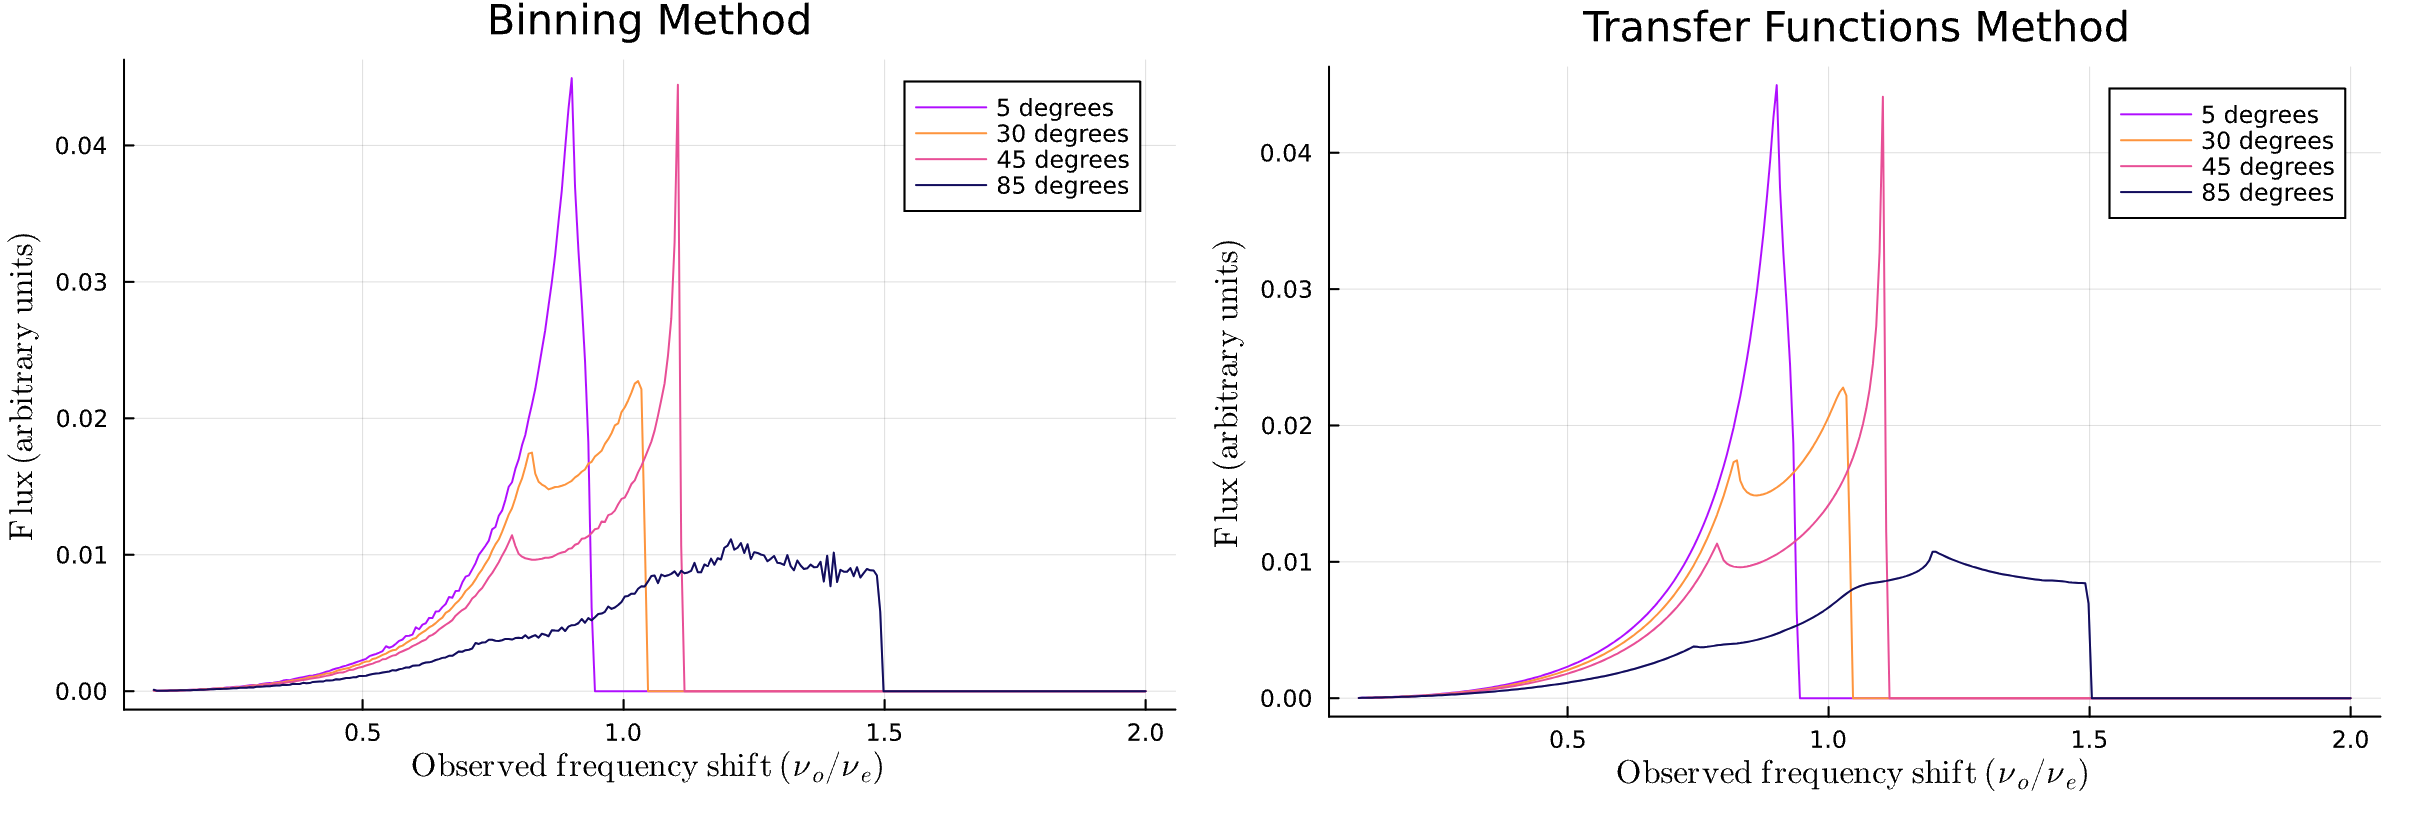
\includegraphics[width=0.98\linewidth]{figures/comparison.png}
    \caption{Comparison of the transfer function method of calculating iron line profiles (right) and the more general binning method (left). Whilst the two are in agreement and give rise to the same line shapes, the binning method exhibits more noise, as expected.}
    \label{comparison}
\end{figure*}

A test was conducted to verify the performance of transfer functions and their accuracy against the binning method as seen in Figure \ref{comparison}. The performance exceeded expectations and the implementation of transfer functions proved correct, confirming the results. For this setup, the same parameters were used as in Figure \ref{fanton} for a Kerr black hole with spin $a = 0.998$ in the {\tt Thin Disc} regime. 

Although the binning method allows for a faster assessment of line profiles, it does exhibit the anticipated noise due to low resolution. Nonetheless, the fundamental shapes of the line profiles remain unchanged, indicating consistency in the methods employed.

The lines rendered by calculations utilising the transfer functions were significantly smoother, especially for profiles perceived by an observer at a high inclination angle. This shows that this method provides a better resolution -- if the same degree of accuracy was expected from the binning method, it would have significantly increased the computation time. Therefore, the transfer function method stands as one providing a better resolution at a lower cost of computation time. This validates the results obtained thus far and supports the utilisation of the transfer functions as a means to calculate the line profiles.

When considering discs with a zero Eddington ratio, a {\tt ThinDisc} model is used instead of the {\tt ShakuraSunyaev}. This allows to better address discrepancies in the intersection algorithm tailored for infinitely thin planes. 

% --> exposing emissivity to coronal spectrum argument
Self-consistent interpretations were calculated utilising the {\tt LampPostModel} included within the {\tt Gradus.jl} software. The model places the isotropic point source at a height $h$ above the black hole in units of $r_{g} = GM/c^{2}$ which is the gravitational radius. 

Initially, the X-ray continuum spectrum due to the presence of corona was dependent on the usual value of the photon index $\Gamma = 2$ \cite{wilkins2012understanding}:
%
\begin{equation}
    \epsilon(r) \approx g^{-\Gamma},
    \label{emissivity}
\end{equation}
%
where $\epsilon(r)$ defines the emissivity and $g$ is the ratio of emitted and observed energy with a detailed calculation outlined in \cite{wilkins2012understanding}.

As a code development element of this work, the emissivity function was exposed to the coronal argument. This allows exploration of how intense the emission is as a function of the disc radius. A new datatype defining an interface of an abstract coronal spectrum was designed as a function taking the {\tt PowerLawSpectrum} type, which defines the dependency on the photon index $\Gamma$, and $g$ as arguments and returns the coronal 
spectrum as $g$ to the power of $\Gamma$. Since the number of photons travelling along any given ray must be conserved for different values of the photon index, it serves as a method to accurately account for any change in the number of photons in each bin of the emissivity profile, with the default value of $\Gamma = 2$, as per \cite{gonzalez2017probing}. 

This new implementation was tested (Figure \ref{test}) by comparing the emissivity profiles created by the function using the default, non-specified spectrum and one with the spectral argument passed on and defined as $\Gamma = 2$.

\begin{figure}
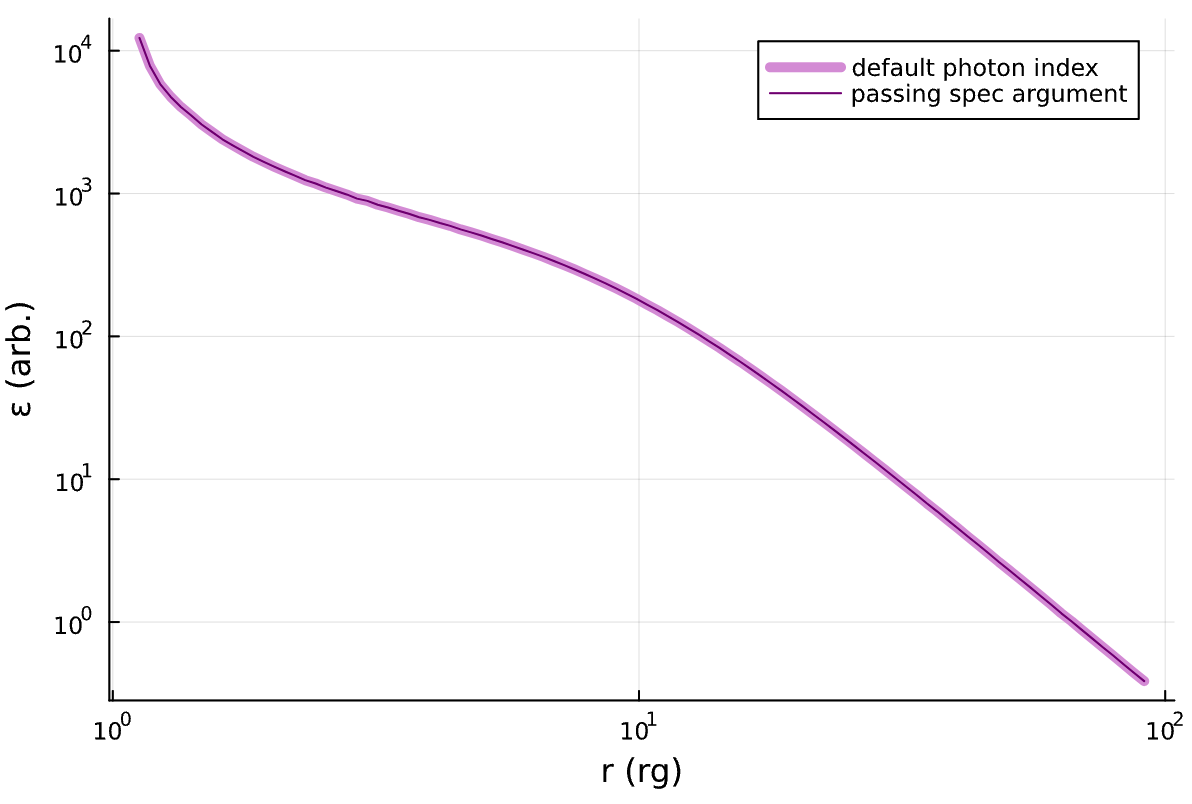
\includegraphics[width=\linewidth]{figures/test.png}
\caption{Visual test comparison of the emissivity profile created using the default setup available in {\tt Gradus.jl} and passing the specified spectrum, which takes the photon index $\Gamma$ as an argument. Since both values were set to 2, the perfect agreement was expected.}
\label{test}
% \end{figure}

% \begin{figure}{l}{0.5\textwidth}
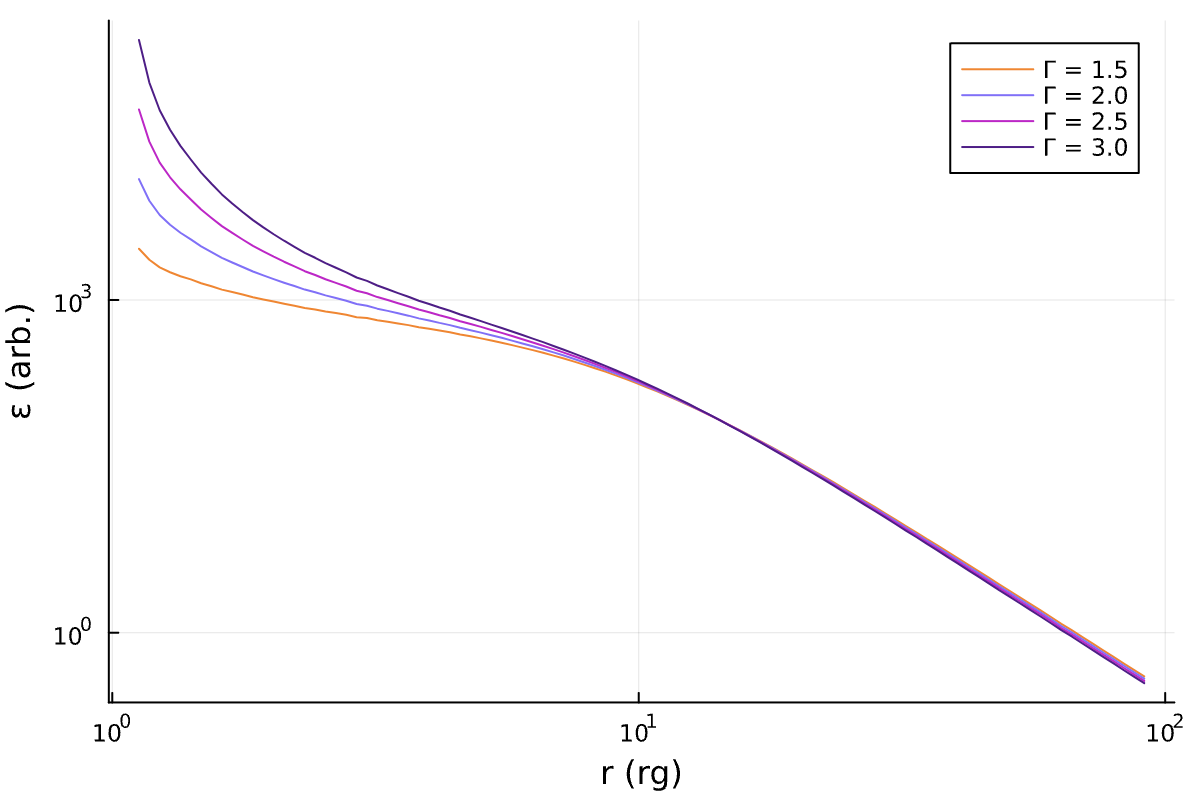
\includegraphics[width=\linewidth]{figures/photonindex.png}
\caption{Results of varying the photon index $\Gamma$ and its impact on the irradiation profile. At small radii, the profile was observed to get more steep as the value of $\Gamma$ was increased. Any differences vanished around $r = 10^{1} r_{g}$.}
\label{photonindex}
\end{figure}

The profiles were expected to be consistent, and so they passed the test. The results in Figure \ref{test} are just a visualisation and a more quantitive comparison of the profiles was performed before the changes were merged into the software.

The photon index was varied between $\Gamma = 1.5, 2.0, 2.5$ and $3$ to investigate its impact on the emissivity profile of the point source as well as to verify consistency with results in the literature (Figure \ref{photonindex}). The model used for this purpose was a maximally rotating Kerr black hole with spin $a = 0.998$ with the lamp post corona located at height $h = 10.0 r_{g}$. 

Results in Figure \ref{photonindex} agree perfectly with those reported in \cite{gonzalez2017probing}. As expected, in the innermost region of the disc, the profile becomes steeper as $\Gamma$ is increased, although this effect vanishes further from this region, becoming minimal around $r = 10^{1} r_{g}$. 

This allowed use of this new version throughout the project, allowing more freedom in choosing the photon index for the calculations of the source to disc emissivity. This is important since the iron lines depend intrinsically on the radial disc profile and such an improvement adds to the completion of the line model if a different $\Gamma$ is of interest. 

% Cross-check between the methods (eg gonzalez wilkins)
%Although not the main objective of this work, 
The profiles can be used as a cross-checking tool between methods. While the results presented in Figure \ref{photonindex} show consistency with the work by \cite{gonzalez2017probing}, as reported in my other work \cite{tarnopolska2024properties}, there are inconsistencies in their aforementioned model when it comes to their other solutions and the results reported in the literature (see \cite{wilkins2012understanding}). Despite that, in those cases which are discussed further in Reference \cite{tarnopolska2024properties}, the results rendered using {\tt Gradus.jl} agreed with those reported by \cite{dauser2013irradiation}.

When considering the self-consistent profiles, the main work of interest was the one by \cite{taylor2018exploring}. To verify the correctness of the self-consistent model used in this work, the effects of varying the height of the corona above the black hole and the disc thickness on the emissivity profile were investigated, with the results presented in Figure \ref{profiletest}.

\begin{figure}
    \centering
    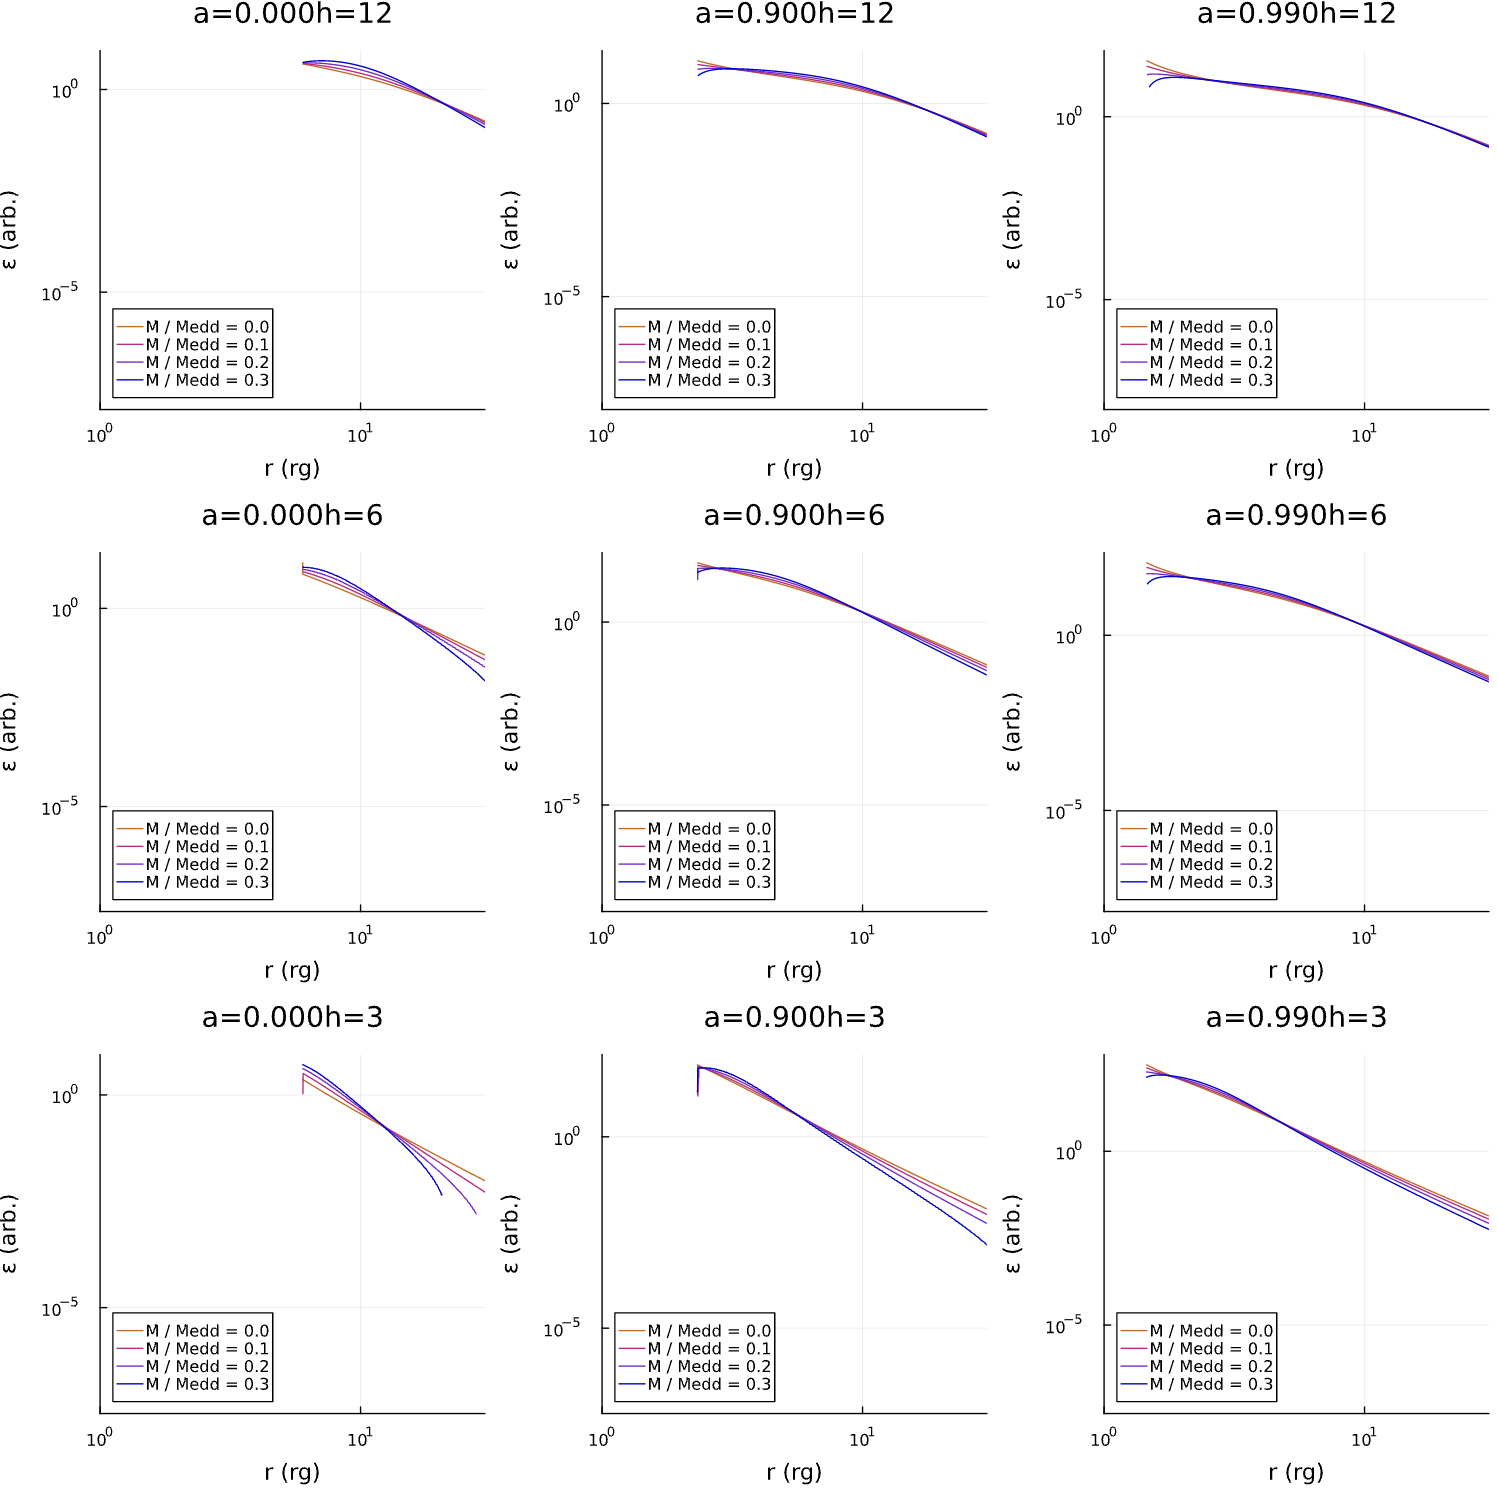
\includegraphics[width=\linewidth]{figures/profiletest.png}
    \caption{Emissivity profiles for various spins, namely $a = 0, 0.9, 0.99$ and coronal heights $h = 3 r_{g}, 6 r_{g}, 12 r_{g}$ for different disc thicknesses $\frac{\dot{M}}{\dot{M}_\text{Edd}}$. The ISCO location was observed to vary with $a$ and the irradiation predicted by the lamp post model of corona heavily depends on the geometry of the disc surface.}
    \label{profiletest}
\end{figure}

Consistently to the literature, as the height of the corona is decreased, more photons hit the disc closer to its innermost part with a decrease in flux observed further on the disc and higher irradiation on the smaller radii on the disc. The drop in the flux is also intrinsically dependent on the coronal height, as particularly visible in the Schwarzschild $a = 0$ case. Additionally, increasing the disc thickness $\frac{\dot M}{M_{\text{Edd}}}$ results in lower photon flux on the outer parts of the disc, followed by the drop moving in closer to the ISCO. 

The drop in emissivity occurs due to disc shadowing \cite{taylor2018exploring} since the increased thickness causes the innermost part of the disc to shield regions further away from the photons emitted by the corona.

Similarly, for higher values of spin, this effect diminishes, which can be explained by the disc thickness decreasing, as per Figure \ref{eddingtonratio}. 

Since both the irradiation and the flux drop depend closely on the coronal height, this proves the coronal geometry critical in accurate determination of the object's emmissivity profile. It also shows that the profile expected of a lamp post corona is surmised to closely depend on the geometry of the surface of the disc, such as its thickness, as well as the geometry of the whole system influenced by the black hole spin.

\newpage

\begin{figure}
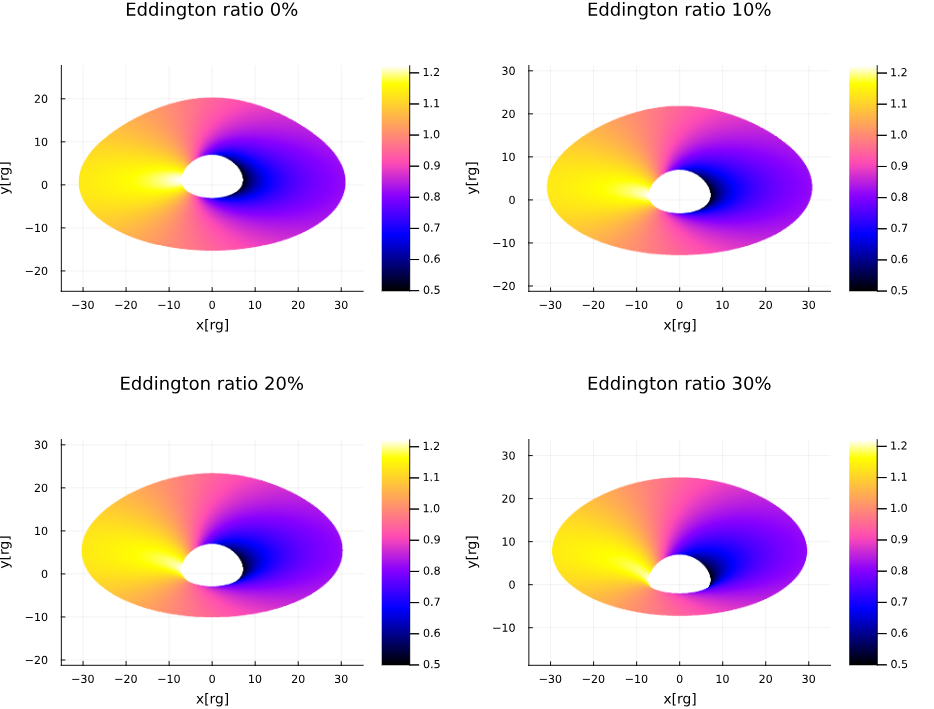
\includegraphics[width=\linewidth]{figures/redshift.png}
\caption{Photon redshift maps traced from the disc to the stationary observer at $r = 10^{3} r_{g}$ and an inclination angle $\theta = 60^{\circ}$ for the case of a Schwarzschild non-rotating black hole. The colourbar visualises the ratio between the energy of the emitted photon and the value observed by the distant observer. As the Eddington ratio is increased, the shape of the disc surface becomes more curved and bowl-like.}
\label{redshift}
\end{figure}

To gain a deeper insight into how the surface geometry of the disc influences the energy of observed photons, photon energy shifts were mapped, as illustrated in Figure \ref{redshift}.

The colour scale corresponds to the ratio of photon energies as emitted by the disc over the energy measured by a distant observer -- the redshift. Here, a case for a non-rotating black hole with spin $a = 0$ was explored for different values of the Eddington ratio $\frac{\dot M}{M_{\text{Edd}}}$ as seen by an observer at a $60^{\circ}$ inclination angle. As expected from a \cite{shakura1973black} disc model, an increase in the Eddington ratio results in the bending of the disc geometry and a more bowl-like shape, as also reported by \cite{taylor2018exploring}. The disc resides flat on the surface for $\frac{\dot M}{M_{\text{Edd}}} = 0$ and becomes more concaved as this value is increased and the disc thickens. The colour map can be interpreted as the material in the yellow part of the disc moving towards the observer (blueshifted) and the blue part moving away (redshifted).

Utilisation of this complex and rigorously tested numerical setup allowed the advancement in  modelling of the black holes iron line profiles as further described.

% --> Recreated Abdikamalov
\section{Power law emissivity}
% POWER LAW
For an irradiation profile following the power law (Equation \ref{intensity}) with the emissivity index $p = 3$ the profile is expected to be sufficiently approximated by $I_{e} \approx \rho^{-p}$. As outlined before, using $\rho$ instead if $r$ is a more appropriate choice to account for the entirety of the disc surface. 

Generally speaking, the influence of the disc thickness is not particularly notable for lower inclination angles, however, it becomes more prominent at higher inclinations. Therefore, the main focus of this section will be a rotating black hole in the Johannsen metric, with varied spin $a$ and deformation parameter $\alpha_{13}$ across different Eddington ratio $\frac{\dot{M}}{\dot{M}_\text{Edd}}$ values as viewed by an observer at $\theta = 70^{\circ}$ inclination as shown in Figure \ref{abdi70}. This essentially replicates the setup presented in \cite{abdikamalov2020testing} describing a black hole in the Johannsen metric, with the inner radius calculated internally using the {\tt Gradus.jl} ISCO function and with the maximum radius ${\tt maxr_{e}}$ set to 500 $r_{g}$.

\begin{figure*}[h!]
    \centering
    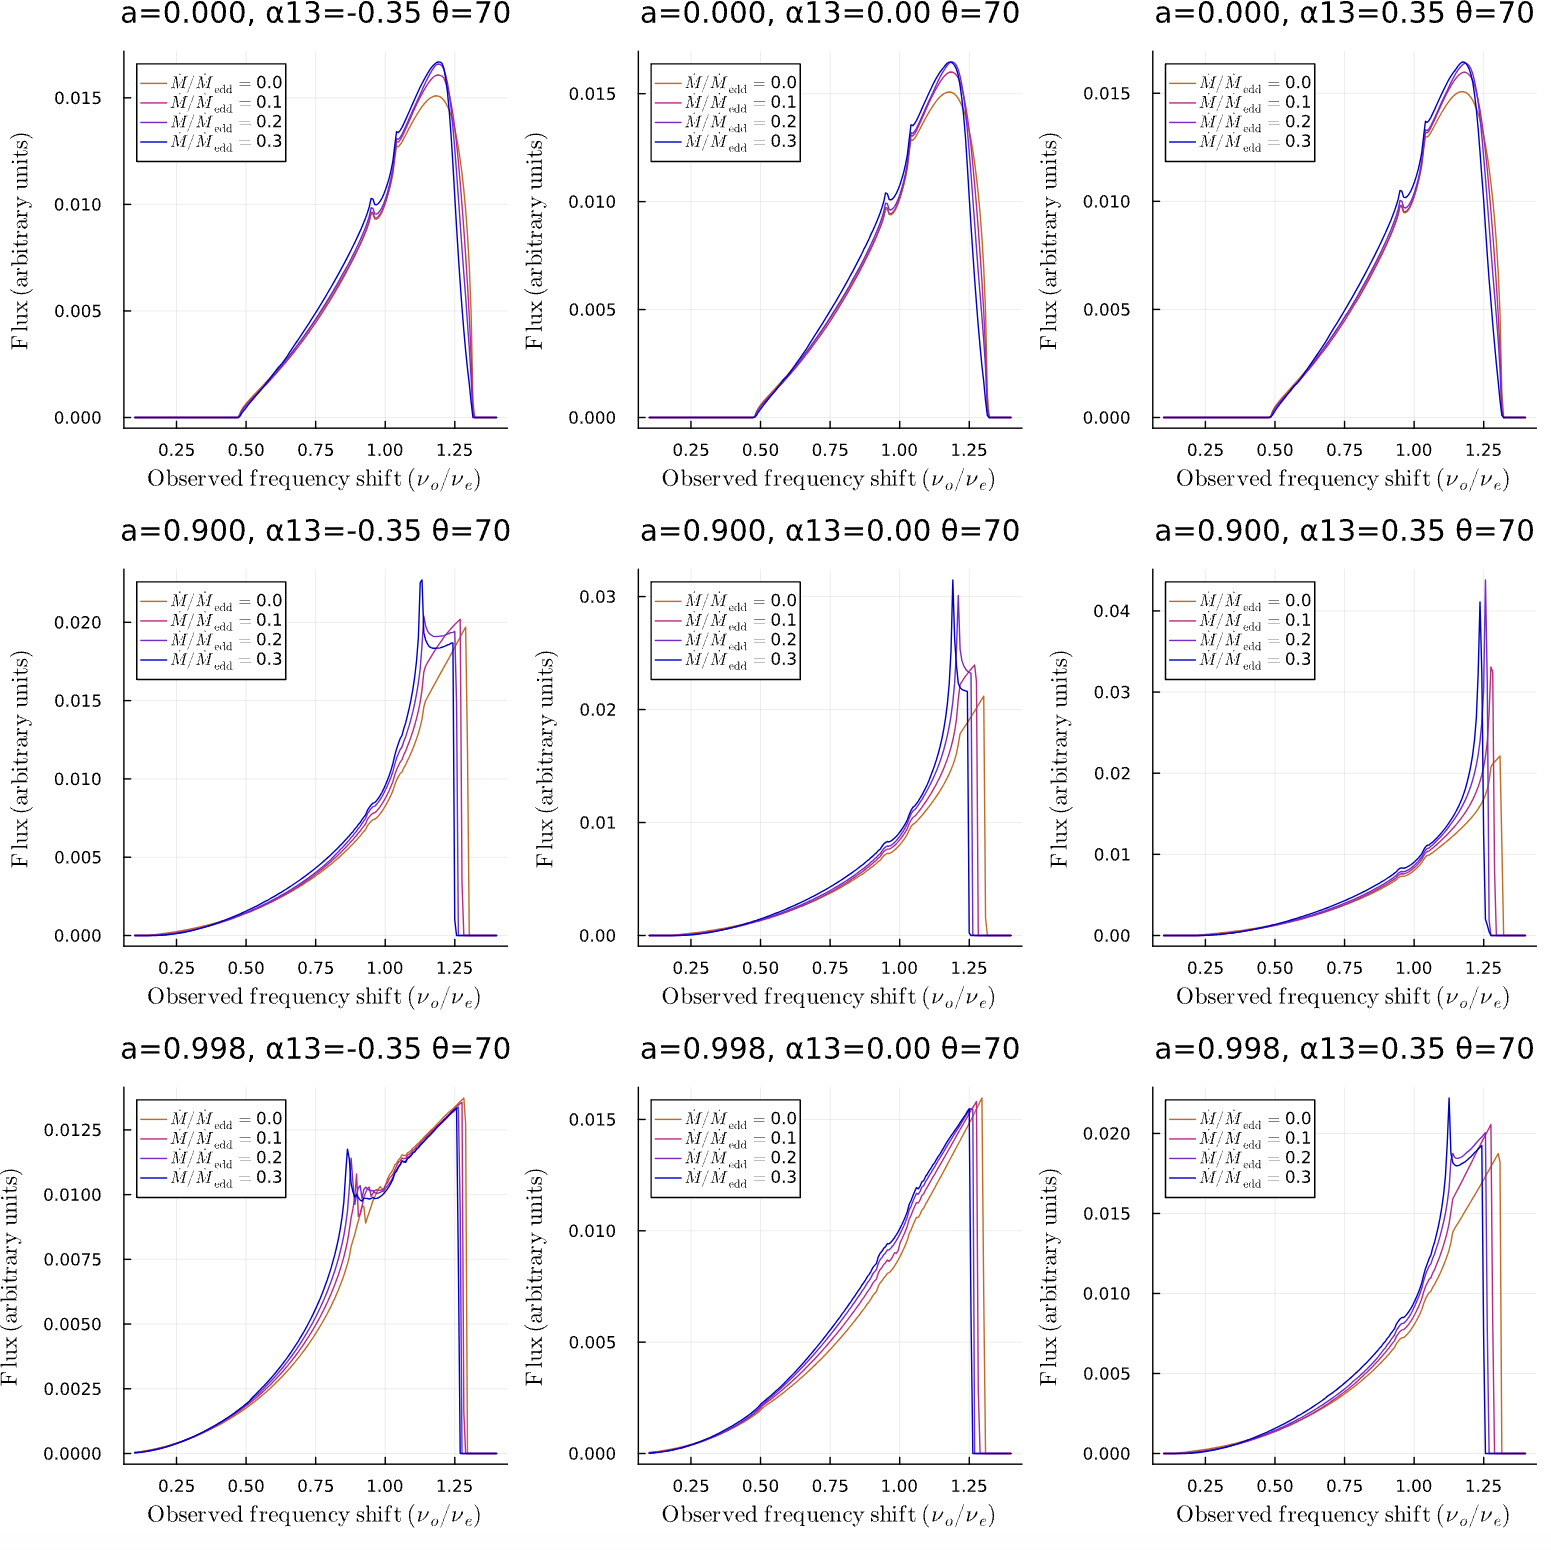
\includegraphics[width=\linewidth]{figures/abdi70.png}
    \caption{Iron line profiles in the Johannsen metric for a black hole with spin $a = 0, 0.9, 0.998$ and deformation parameter $\alpha_{13} = -0.35, 0, 0.35$ as viewed by an observer at $\theta = 70^{\circ}$ inclination. Shows the profiles for discs of different thicknesses $\frac{\dot M}{M_{\text{Edd}}}$.}
    \label{abdi70}
\end{figure*}

As the spin is increased, broadening of the iron line profile is observed for all values of $\alpha_{13}$, although for the deformation parameter itself, no clear trend was noted when considering differences across discs of varied thickness. Interestingly, a distinguishable peak was discovered in the Kerr ($\alpha_{13} = 0$) solution when $a = 0.9$ which declines at spin increases up to the maximum $a = 0.998$ value. The same feature was reported by \cite{abdikamalov2020testing}. While the changes on $\alpha_{13}$ do not follow a clear trend as far as disc thickness is concerned, they do impact the overall shape of the iron line profile and appear to shift the peak flux upwards. Eddington ratio on the other hand, and therefore the disc thickness, typically results in a lower photon flux at the peak of the line profile as it decreases. At higher values of spin, the observed effects due to the deformation parameter are more pronounced -- in those cases, increasing the disc thickness tends to move the peak down to lower observed frequency shifts, which correspond to lower energies. This result is consistent with literature \cite{abdikamalov2020testing}.

% SELF CONSISTENT
\section{Self--consistent emissivity}

\begin{figure*}[h!]
    \centering
    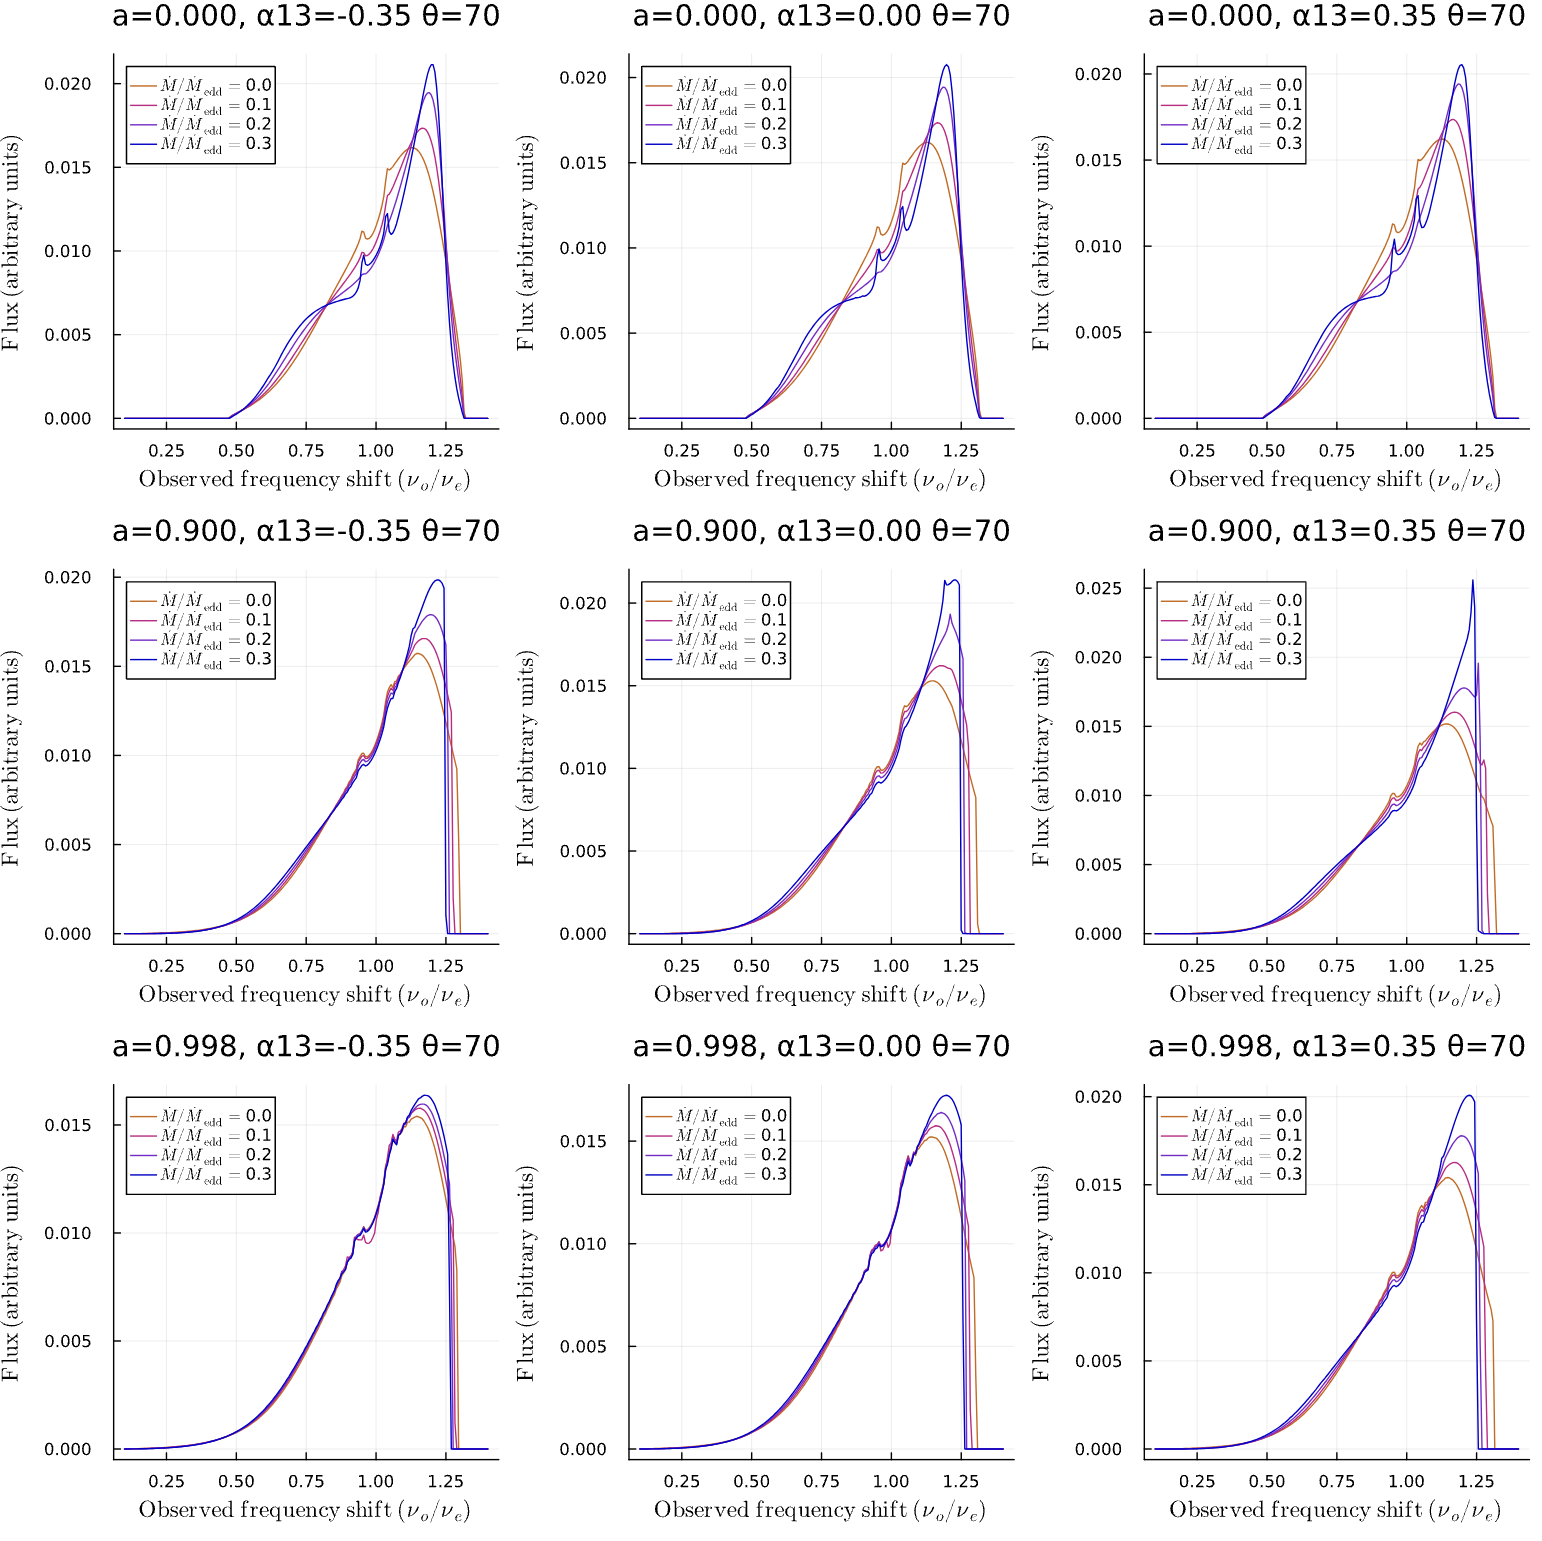
\includegraphics[width=\linewidth]{figures/selfconsistent_abdi70.png}
    \caption{Same as Figure \ref{abdi70} but modelled self-consistently with using a lamp post model of corona at height $h=10 r_{g}$ and a photon index $\Gamma = 2$.}
    \label{selfconsistent_abdi70}
\end{figure*}

% SELF CONSISTENT Abdikamalov
The same setup as in Figure \ref{abdi70} was also reproduced in the self-consistent regime using a lamp post model of the corona at height $h=10 r_{g}$ and a photon index $\Gamma = 2$, which is the default value, in Figure \ref{selfconsistent_abdi70}. 

The self-consistent approach yielded different results than the power law approximation method. Whilst the differences do not become more pronounced between different values of $\alpha_{13}$ for a non-rotating case, additional spikes were observed at higher Eddington ratios. The peak becomes more spiked with the increased deformation parameter, especially for a thicker disc at $a = 0.9$. The most striking changes between different values of $\frac{\dot{M}}{\dot{M}_\text{Edd}}$ were observed for the maximum spin $a = 0.998$ case.  Notably, as the value of $\alpha_{13}$ is increased, a larger difference in the maximum flux is observed for different Eddington ratios.

\begin{figure*}[h!]
    \centering
    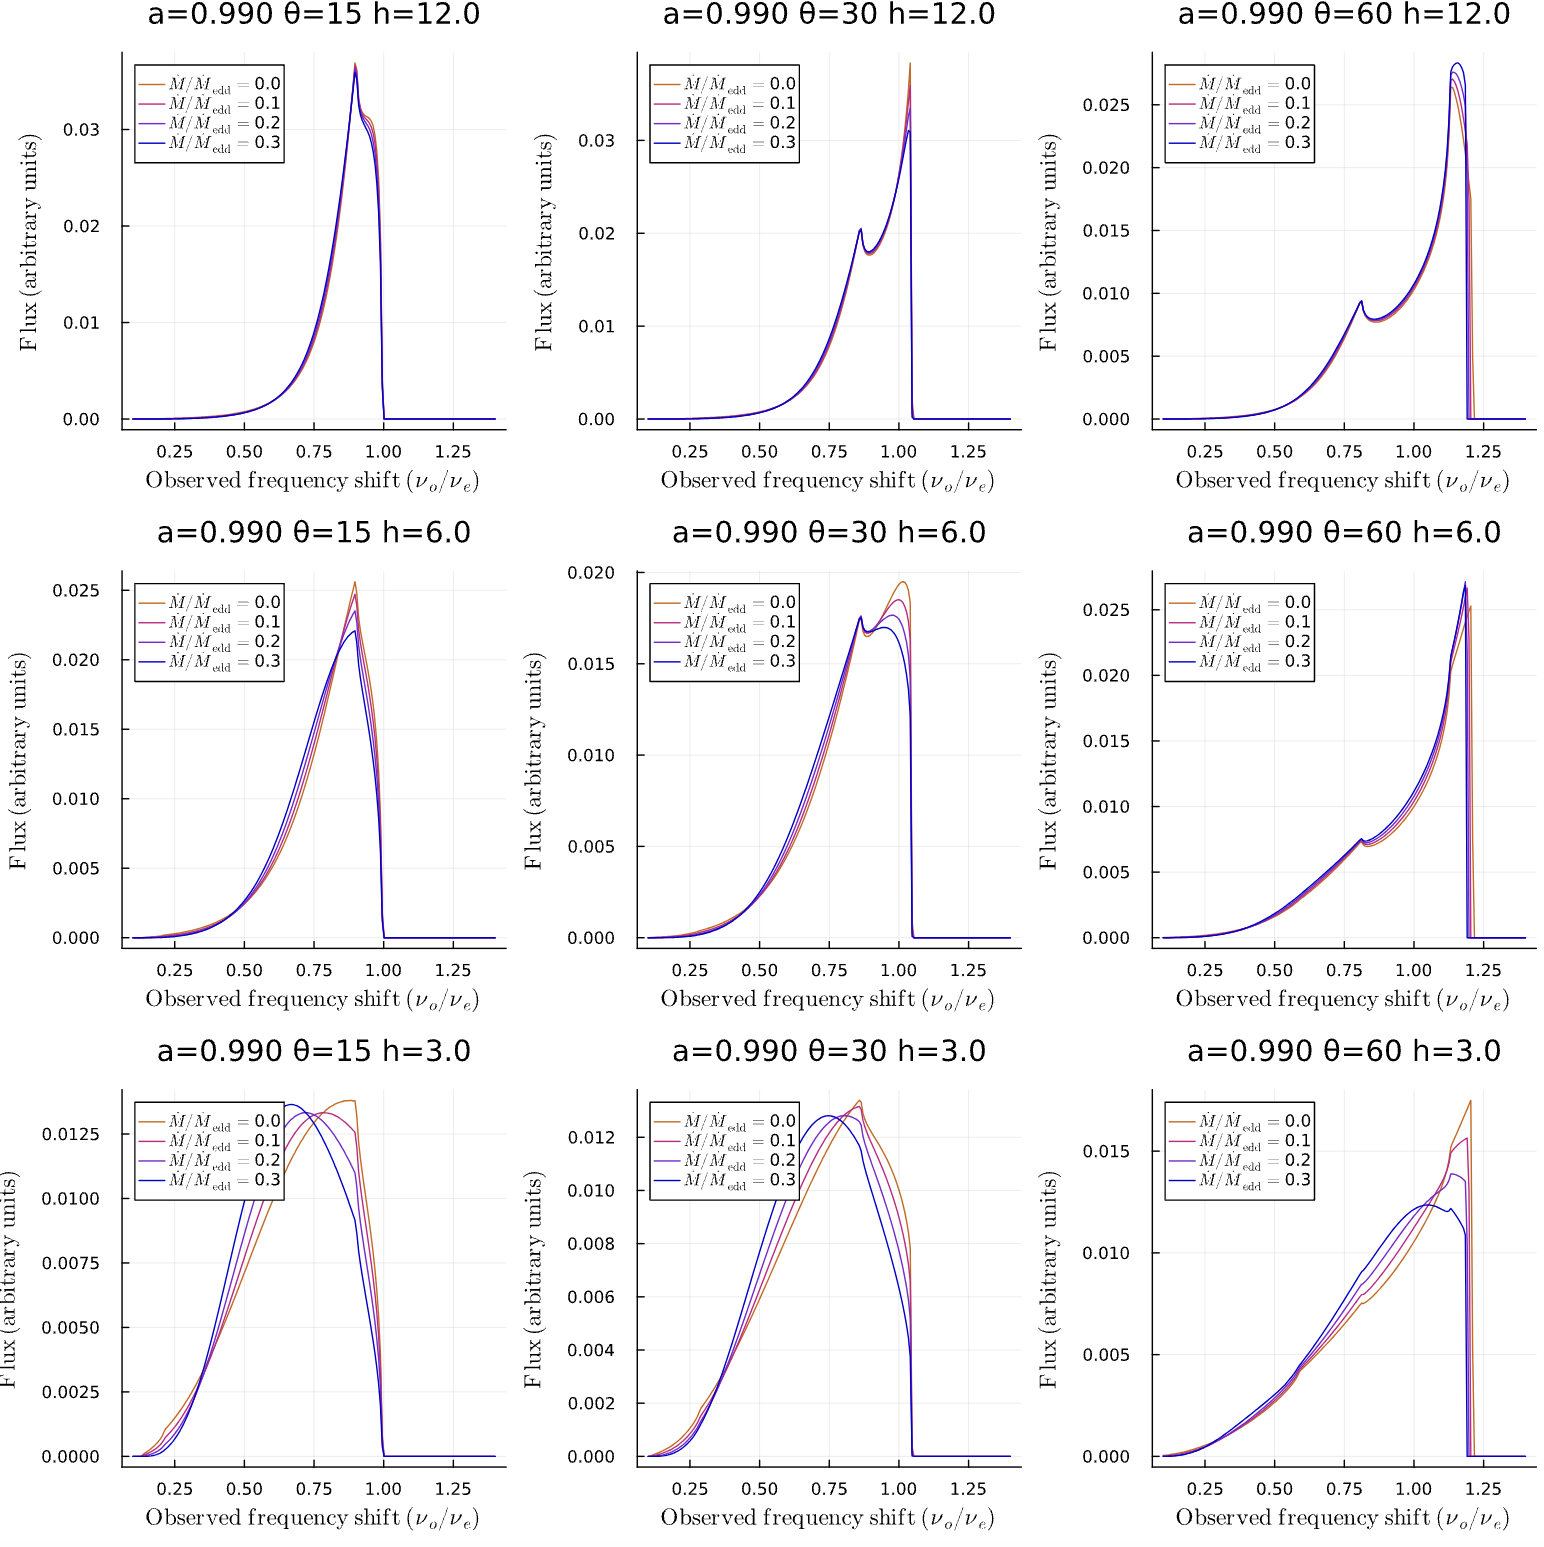
\includegraphics[width=\linewidth]{figures/taylorreynolds.png}
    \caption{Iron line profiles for a rapidly rotating black hole with spin $a = 0.99$ at inclinations $\theta = 15^{\circ}, 30^{\circ}, 60^{\circ}$. The effects of geometry were observed to become more pronounced as the coronal height $h$ was decreased.}
    \label{taylorreynolds}
\end{figure*}

% --> Recreated Taylor Reynolds
Moving forward with the conclusion that the most pronounced relativistic effects for various Eddington ratios occur for high values of spin $a$, the results of varying the height of a lamp post corona were simulated. Here, the ${\tt minr_{e}}$ was again calculated using the ISCO function dependent on the metric and the outer ${\tt maxr_{e}}$ radius was set to 30 $r_{g}$ in an attempt to recreate the setup outlined in Reference \cite{taylor2018exploring}.

Figure \ref{taylorreynolds} shows the outcome of this model for a rapidly rotating black hole with spin $a = 0.99$ in the Kerr metric. The effects of geometry were the weakest for the largest height investigated, $h = 12 r_{g}$, and increased as the corona was lowered down. As the height $h$ of the corona above the black hole decreased, the line shapes broadened due to gravitational effects.

Additionally, for the lowest $h = 3 r_{g}$ case, the most noticeable effects were observed between different values of $\frac{\dot{M}}{\dot{M}_\text{Edd}}$. Particularly at higher inclinations, low-placed corona caused the flux to decrease with increasing disc thickness.

Furthermore, for the low $\theta = 15^{\circ}$ and moderate $\theta = 30^{\circ}$ inclination angles and corona placed low above the black hole at $h = 3 r_{g}$ there appears to be a shift of the iron line peak towards lower energies (lower observed frequency shifts) as the Eddington ratio is increased, while for a high $\theta = 60^{\circ}$ inclination case, this trend appeared to be less pronounced.

%johannsen self-consistent, varied height
\begin{figure}
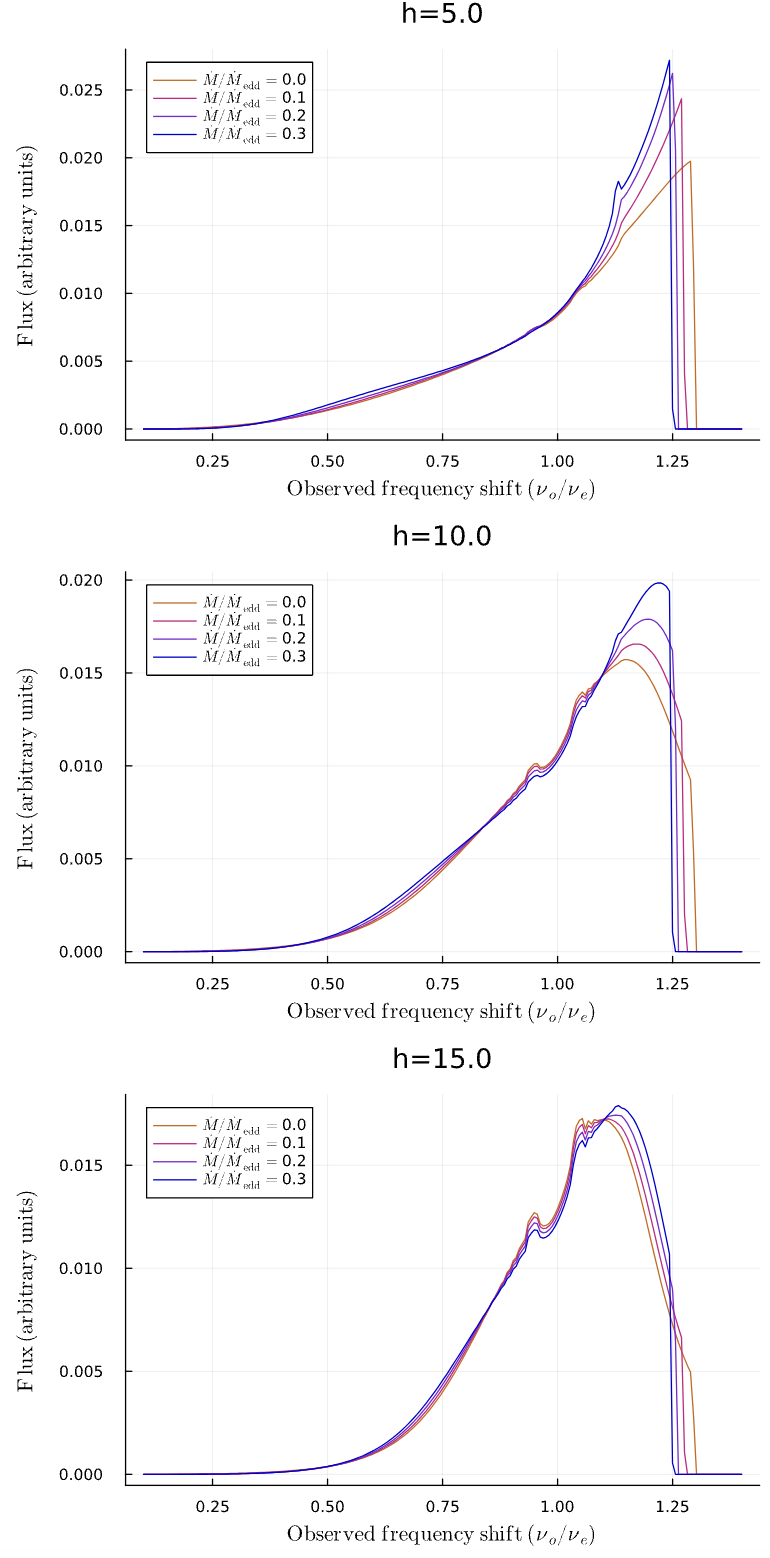
\includegraphics[width=\linewidth]{figures/johannsen_selfconsistent.png}
    \caption{Iron line profile for a black hole with spin $a = 0.9$ and deviation parameter $\alpha_{13} = -0.35$ for corona located at height $h = 5, 10, 15  r_{g}$.}
    \label{johannsen_selfconsistent}
\end{figure}

% --> Johannsen self-consistent
Drawing from both \cite{abdikamalov2020testing} and \cite{taylor2018exploring} a few conclusions can be made already. Interesting cases occur for rapidly rotating black holes, specifically viewed at high inclination angles. Furthermore, while the Kerr metric can be modelled self-consistently, the Johannsen metric \cite{johannsen2013regular} has only ever been modelled using the power law approximation. As has been shown so far, the geometry of the system can significantly impact its behaviour as a whole, causing pronounced changes in the iron line profiles as the geometry of the lamp post model of the corona is varied. Specifically, for a point source located close to the accretion disc, the differences between discs of different thicknesses become particularly noticeable. 
Utilising this knowledge, an advancement was made in simulating the Johannsen metric self-consistently, while varying deformation parameters for the first time as follows.


Figure \ref{johannsen_selfconsistent} shows the effects of varying the height of the isotropic point source corona above the disc in the Johannsen metric with one non-zero deformation parameter $\alpha_{13} = -0.35$ for a rapidly rotating black hole with spin $a = 0.9$ and the observer at an inclination angle $\theta = 70^{\circ}$. 

As expected, the result was a higher maximum flux for the point source located lower above the black hole. The line profiles appear to typically shift the peak towards lower energies as the coronal height increases. The shape of the line changes significantly with height, and the differences in maximum flux across different Eddington ratios decrease with increasing $h$.

% multiple deformation parameters varied example
\begin{figure*}
    \centering
    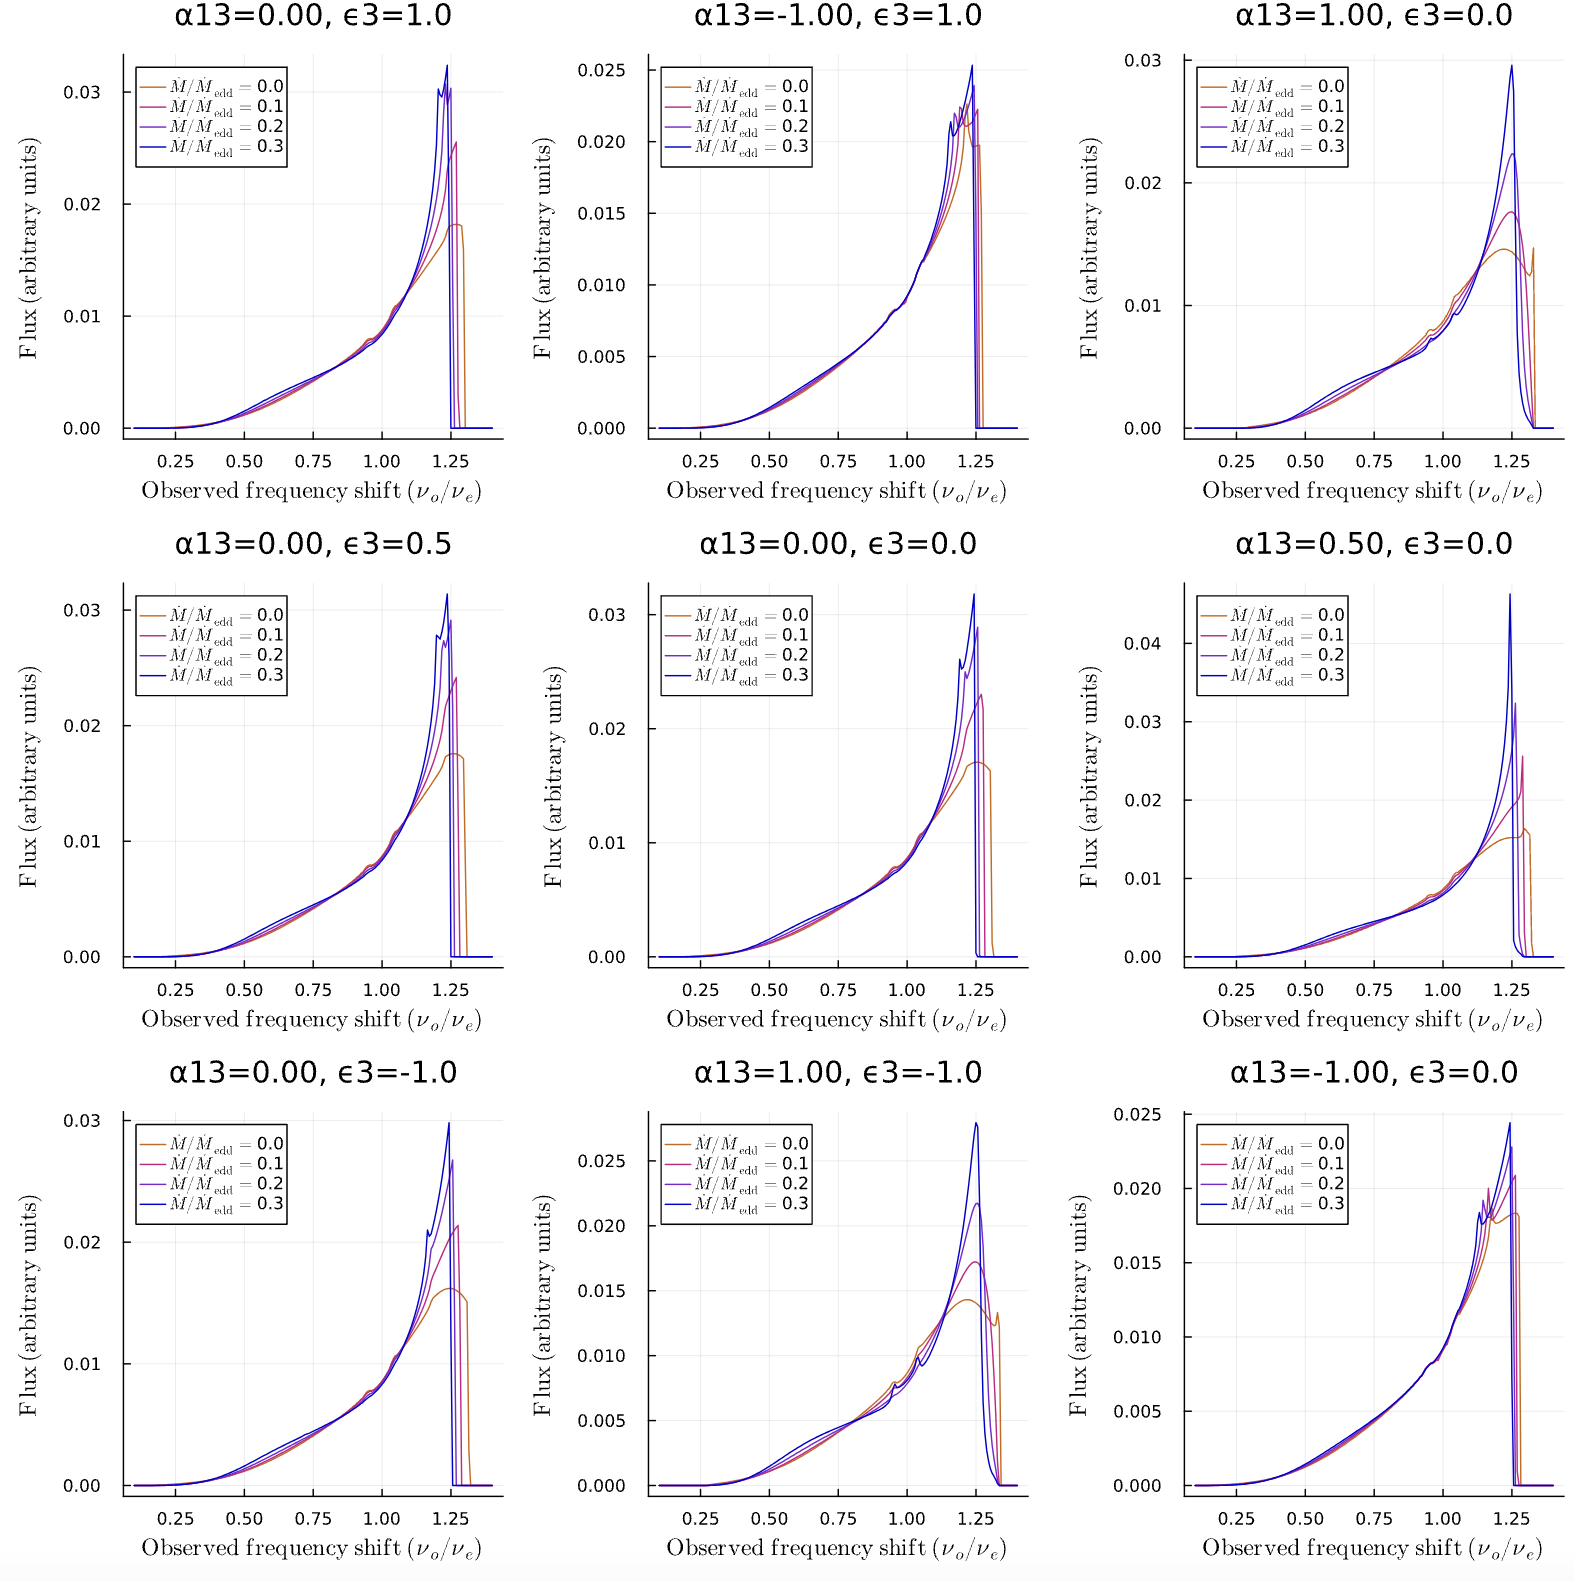
\includegraphics[width=0.98\linewidth]{figures/johannsen_deformation.png}
    \caption{Iron line profiles in the Johannsen metric modelled self consistently for the first time. The left column shows the effects of varying $\epsilon_{3}$ while keeping $\alpha_{13} = 0$ constant, the middle column -- both parameters varied simultaneously and the right column with varying $\alpha_{13} = 0$ and keeping $\epsilon_{3} = 0$ with the corona located at $h = 6 r_{g}$ and the photon index $\Gamma = 2$}
    \label{johannsen_deformation}
\end{figure*}

A further novelty of the model was to self-consistently simulate the variation of multiple deformation parameters -- namely $\alpha_{13}$ and $\epsilon_{3}$ as depicted in Figure \ref{johannsen_deformation} for a black hole with spin $a = 0.9$, the corona located at $h = 6 r_{g}$ with the photon index $\Gamma = 2$ and the observer at the inclination angle $\theta = 70^{\circ}$. The figure shows the effect of changing $\epsilon_{3}$ whilst keeping $\alpha_{13} = 0$, simultaneous changing of both of those parameters as well as varying $\alpha_{13}$ whilst $\epsilon_{3}$ is kept as zero in consistency with conditions for the deviations parameters introduced in Equations \ref{alpha13} and \ref{epsilon3}. 

Decreasing $\epsilon_{3}$ appears to be shifting the iron line flux peak lower across all Eddington ratios in this case. As before, variation of $\alpha_{13}$ does not follow any specific trend when it comes to the height of the disc, although the maximum flux differences appear to increase with the parameter.  Interestingly, if $\alpha_{13} = -1$ and $\epsilon_{3} = 1$, the difference in maximum flux for discs with different thicknesses is not as pronounced, although becomes more significant if the values are swapped. It also appears for the $\alpha_{13} = 1$ and $\epsilon_{3} = -1$ case, that as the $\frac{\dot{M}}{\dot{M}_\text{Edd}}$ is increased, the blue wing becomes taller. The dependence of flux on the thickness of the disc becomes more noticeable, with extra peaks appearing for thicker discs. 

% -->Degeneracies in iron line profiles (johannsen)
\section{Iron line profiles degeneracies}

\begin{figure*}
    \centering
    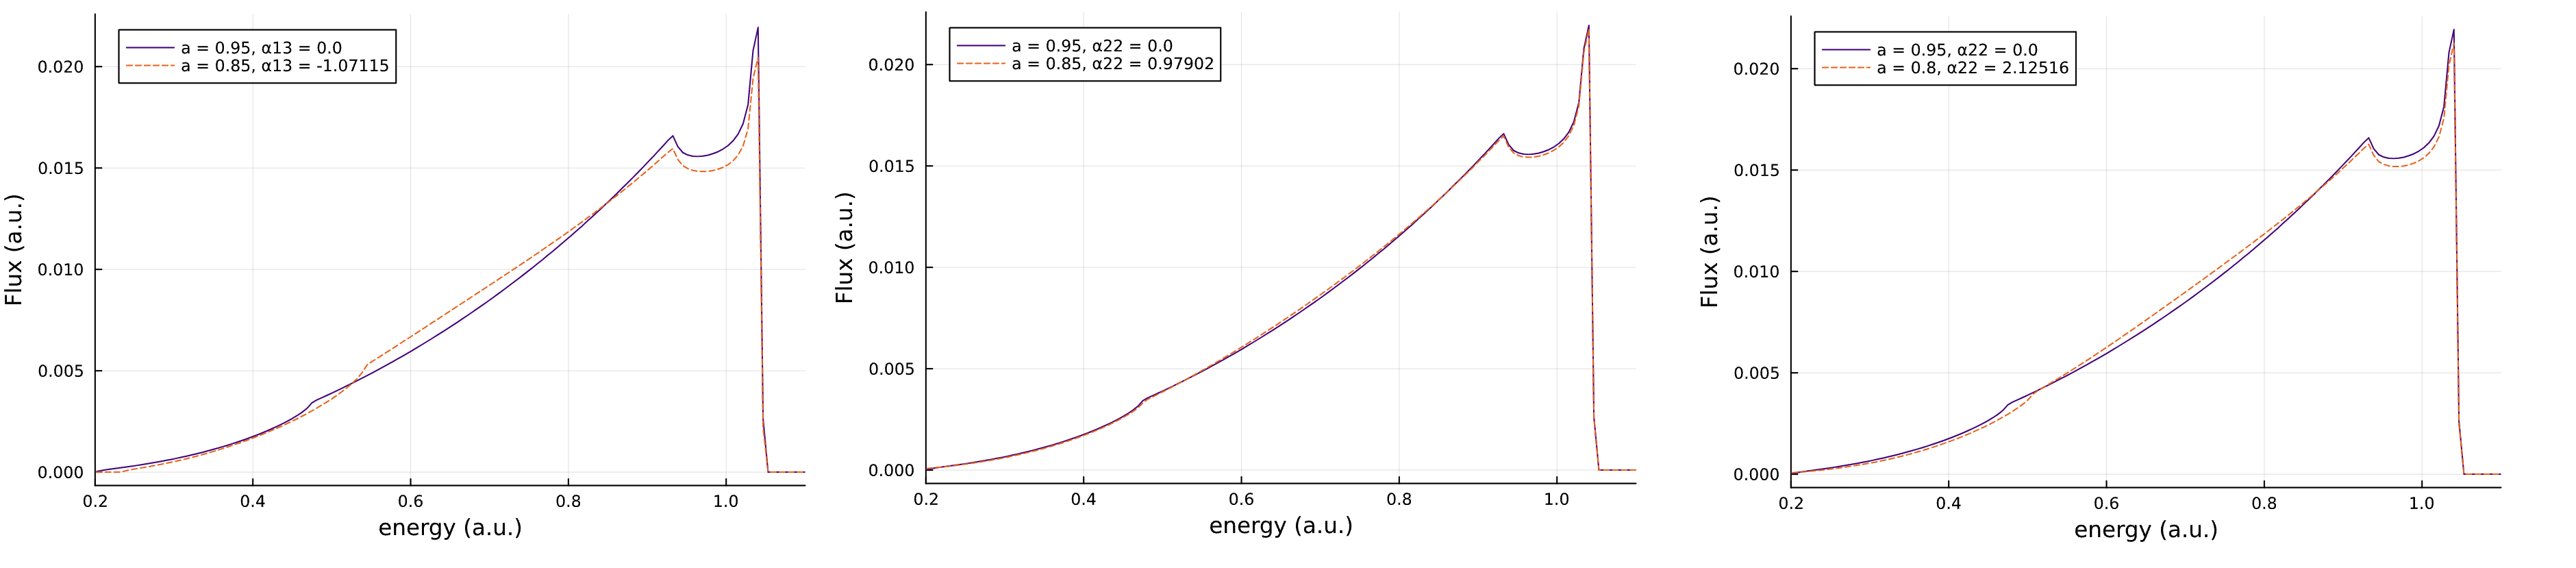
\includegraphics[width=0.98\linewidth]{figures/johannsen_h10_Gamma3.png}
    \caption{h = 10, $\Gamma = 3$}
    \label{johannsen_degeneracy}
\end{figure*}

An interesting observation reported in \cite{johannsen2014x} is that once the deformation parameters are introduced, the black holes that are not described by the same set of variables can give rise to identical broadened iron line profiles.

As outlined in Reference \cite{johannsen2014x}, the effect of deviation parameters $\alpha_{13}$ and $\alpha_{22}$ is very similar. When the $\alpha_{13}$ parameter is increased and $\alpha_{22}$ is decreased, the fluxes of the two peaks increase and the tail of the iron line is shortened. The dependency on the other two deviation parameters -- $\epsilon_{3}$ and $\alpha_{52}$ is marginal in comparison.

While the profiles might look identical despite different spins when the deviation parameters are at play, giving rise to \textit{degeneracies}, this is only applicable to black holes with low to intermediate values of spin $a$. For rapidly rotating black holes, the differences become more pronounced if the parameters are set to high enough values\cite{johannsen2014x}. 

The results reported by \cite{johannsen2014x} rely on the broken power method to calculate the illumination patterns of the disc. As shown previously in this work, the impact of the coronal geometry is intrinsically related to the iron line profile shape. Therefore, the same effects of varying deformation parameters on the degeneracy of the line profiles were modelled in the self-consistent approach.

Effects of variation of different deformation parameter are displayed in Figure \ref{johannsen_degeneracy} for a black hole viewed by an observer at the inclination angle $\theta = 30^{\circ}$ in the self-consistent approach with a point source corona located at height $h = 10 r_{g}$ above the black hole with an accretion disc spanned between the ISCO and ${\tt maxr_{e}} = 100 r_{g}$ and the photon index $\Gamma = 3$, recreating the setup in Reference \cite{johannsen2014x}.


These results are perfectly consistent with those stated by Johannsen, despite using the self-consistent lamp post geometry. Not only do the figures match perfectly, they also prove the previously stated effects of the deformation parameters $\alpha_{13}$ and $\alpha_{52}$ on the shapes of the iron line profiles. Furthermore, the degeneracy is shown to occur for a set of two black holes, one with spin $a = 0.95$ and $\alpha_{22} = 0.0$ and the second with $a = 0.85$, $\alpha_{22} = 0.97902$.


\section{Discussion} 
% Abdikamalov2020 power law 
When discussing the effect of disc thickness on the iron line profile shape, \cite{abdikamalov2020testing} attribute it to the stronger gravitational field if the ISCO is in close vicinity of the black hole, which occurs for higher spins, as per Figure \ref{height}. This is expected to lead to more pronounced effects on the profile, even if the deviations from the original emission point are minor. However, the proximity of the black hole results in higher radiative efficiency $\eta$, hence making the disc \textit{thinner} and giving rise to smaller discrepancies when compared to a razor-thin disc model. This can be observed about results presented in Figure \ref{abdi70}. The differences for various disc thicknesses are more pronounced for $a = 0.9$ than $a = 0$, although for a maximally rotating black hole $a = 0.998$, they were observed to be less prominent due to disc flattening.

The peaky feature observed in Figure \ref{abdi70} for $a = 0.9$ and the deformation parameter $\alpha_{13} = 0$ was not observed for the thin ($\frac{\dot{M}}{\dot{M}_\text{Edd}} = 0$) disc and was particularly pronounced for models with higher Eddington ratios in discs with finite thickness. It is explained in the Reference \cite{abdikamalov2020testing} to be closely related to the aforementioned phenomenon of the disc obscuring itself (self-shadowing), which becomes particularly significant at high inclination angles, alongside with the Doppler boosting. The feature disappears again for a maximal possible spin due to the disc being thinner due to higher $\eta$ as outlined before. 

% self-consistent Abdikamalov
In the self-consistent approach no peaky features resembling those were observed, implying it is dependent on the model and whether a coronal geometry is implemented or if the illumination pattern is approximated using power law. However, additional peaks were observed for thicker discs at $\frac{\dot{M}}{\dot{M}_\text{Edd}} = 0.3$ of a Schwarzschild black hole (Figure \ref{selfconsistent_abdi70}. 
% why????
While for the non-rotating black hole, the differences across different values of the deviation parameter $\alpha_{13}$ remain non-observable, it appears to sharpen the peaks of the rotating black holes as its value is increased. Additionally, the maximum flux increases across all Eddington ratios due to the increase in $\alpha_{13}$, which according to Reference \cite{johannsen2014x} is caused by the orbital velocity of the accretion flow. 

In the case of both the power law and the self-consistent approach, the red peak remained fairly unaffected whilst the most identifiable difference due to variation of $\alpha_{13}$ was observed on the blue peak. This result had been observed before in the literature \cite{johannsen2014x}, \cite{johannsen2013testing} and implies a possible test of the no-hair theorem by comparing the flux difference between the two peaks. Although this is a promising application, the red peak is often difficult to identify from the line profile as the geometry of the system varies and the redshifted peak can get absorbed into the line and become harder to identify. 

% Taylor Reynolds 2018 spins / heights
For a rapidly rotating $a = 0.99$ black hole, the effects due to the coronal geometry of the system were the most pronounced for the corona located at height $h = 3$, decreasing as the corona was set further away as shown in Figure \ref{taylorreynolds}. As these effects become more prominent at low and moderate coronal heights, an overall decrease in peak line flux was observed for increasing disc thickness with the most prominent suppression occurring at the high inclination angle $\theta = 60^{\circ}$ for a corona located low above the black hole. Additionally, the energy of the peak shows dependency on the disc thickness parameter, overall decreasing for higher values of the Eddington ratio at low and moderate inclinations, although this particular effect became less pronounced at high inclination.

\begin{figure*}
    \centering
    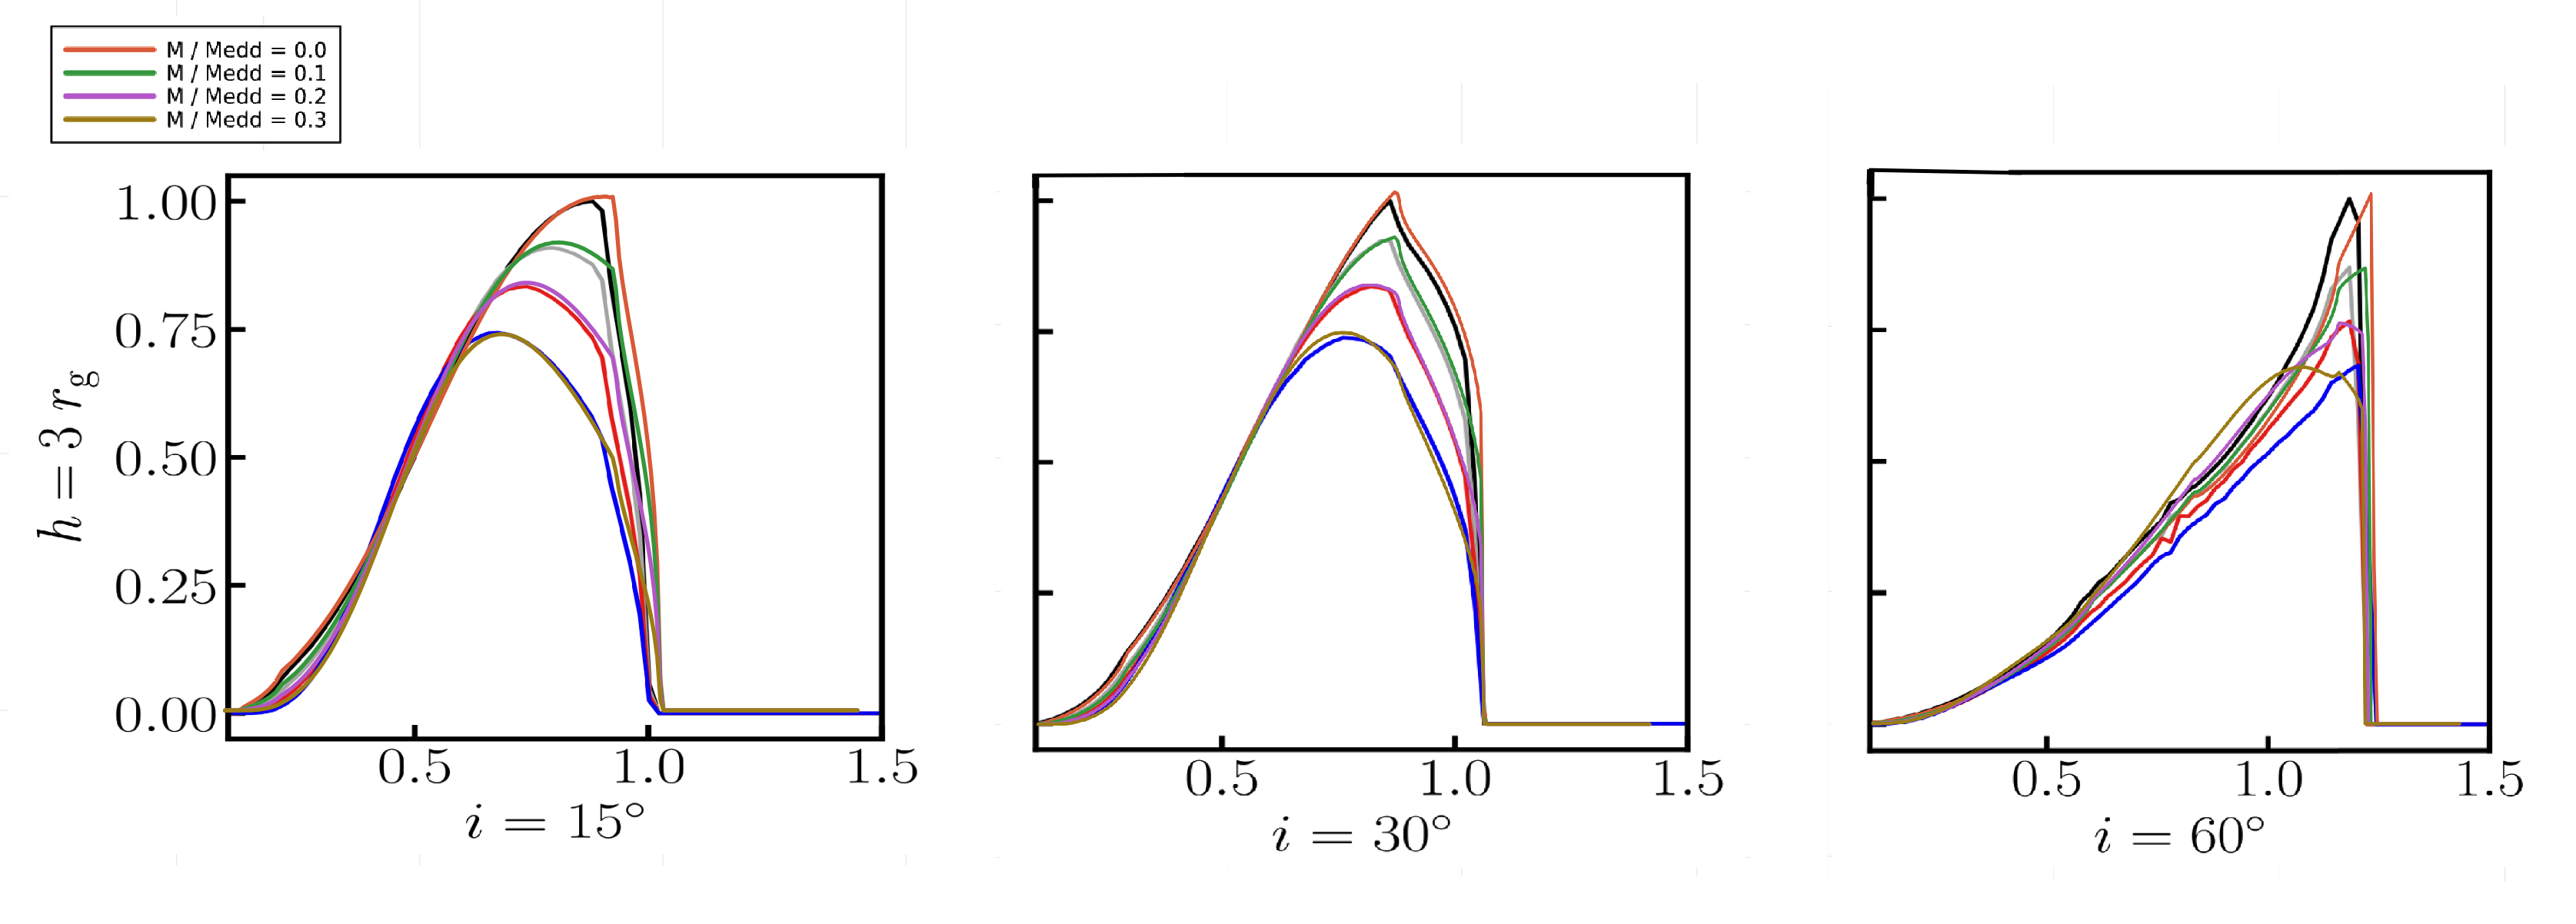
\includegraphics[width=0.98\linewidth]{figures/overlay.png}
    \caption{Results from overlaying the low coronal height $h = 3 r_{g}$ case from Figure \ref{taylorreynolds} over the results from \cite{taylor2018exploring} work. The discrepancy between the plots appears to propagate and intensify with increased inclination angle and disc thickness.}
    \label{overlay}
\end{figure*}

% use overlay?
Comparing these results with the work of Taylor \& Reynolds \cite{taylor2018exploring}, whilst the line profiles appear to agree in the overall shape and the trends followed, particularly notable differences were observed for cases at low height. Using the method of overlaying images it was possible to directly compare the plots. In fact, it was found that the difference for low and moderate inclinations at low coronal height was primarily due to the normalisation implemented in Reference \cite{taylor2018exploring} and which was found by trial and error with respect to the highest peak. Figure \ref{overlay} shows the overlay of the plots and their satisfactory agreement at low and moderate inclinations. However, a significantly more pronounced discrepancy was noted for the higher inclination case with the most pronounced difference in the observed line profile shape at $h=3 r_{g}$, particularly for the thicker disc cases. Notably, the plots being reported in this work were more curved and the blue peak was less sharp. 

It is those high spin combined with high inclination cases that are most interesting from the research point of view. Supermassive black holes residing at the centres of most galaxies (AGNs) are reported to be dominated by rapidly rotating compact objects\cite{reynolds2015measuring}.

Higher inclination angles were chosen in this work due to them making the numerical problems most pronounced. Whilst our method gave a good agreement at lower inclinations, high inclinations showed more prominent differences between our model and the one implemented in the Reference \cite{taylor2018exploring}. This further highlights the need for more than one independent numerical framework to reproduce results. Since the code used by \cite{taylor2018exploring} is not publicly available it is difficult to determine the specific source of discrepancies. The setup was replicated identically and since the {\tt Transfer Functions} method was tested and proved to perfectly agree with the {\tt Binning Method} it is definitely not a method fault. Furthermore, the transfer function integration in principle does not account for the false image since it cannot be observed and was therefore hard-coded to be disabled. The area inside the ISCO, where the false images might emerge, is believed to be completely opaque because of the intense ionization, and thus, does not affect the line profile. Suspecting the model in literature may have included the false image it was enabled and tested using the binning method in line profile calculation, but the difference persisted.

Analysing Figure \ref{overlay}, it can be observed that even for the thin disc with a zero Eddington ratio the profiles do not match exactly. The discrepancy intensifies for thicker discs. When it comes to flux contribution in the line profile, it is mainly the radiation from the innermost parts of the disc that influences the shape of the inner and outer parts of the line. Any contribution from the intermediate parts can be seen in the middle of the profile shape, although this is less significant. The main area of interest is therefore close to the central black hole where the relativistic effects are the strongest. Given that the binning method was used in Reference \cite{taylor2018exploring} and the {\tt Binning Method} in {\tt Gradus.jl} matches perfectly with the {\tt Transfer Function} method, it became possible that a different plane might have been implemented in the aforementioned work. Figure \ref{grid} shows two different types of grids used in the binning method -- the linear and geometric grid.

\begin{figure*}
    \centering
    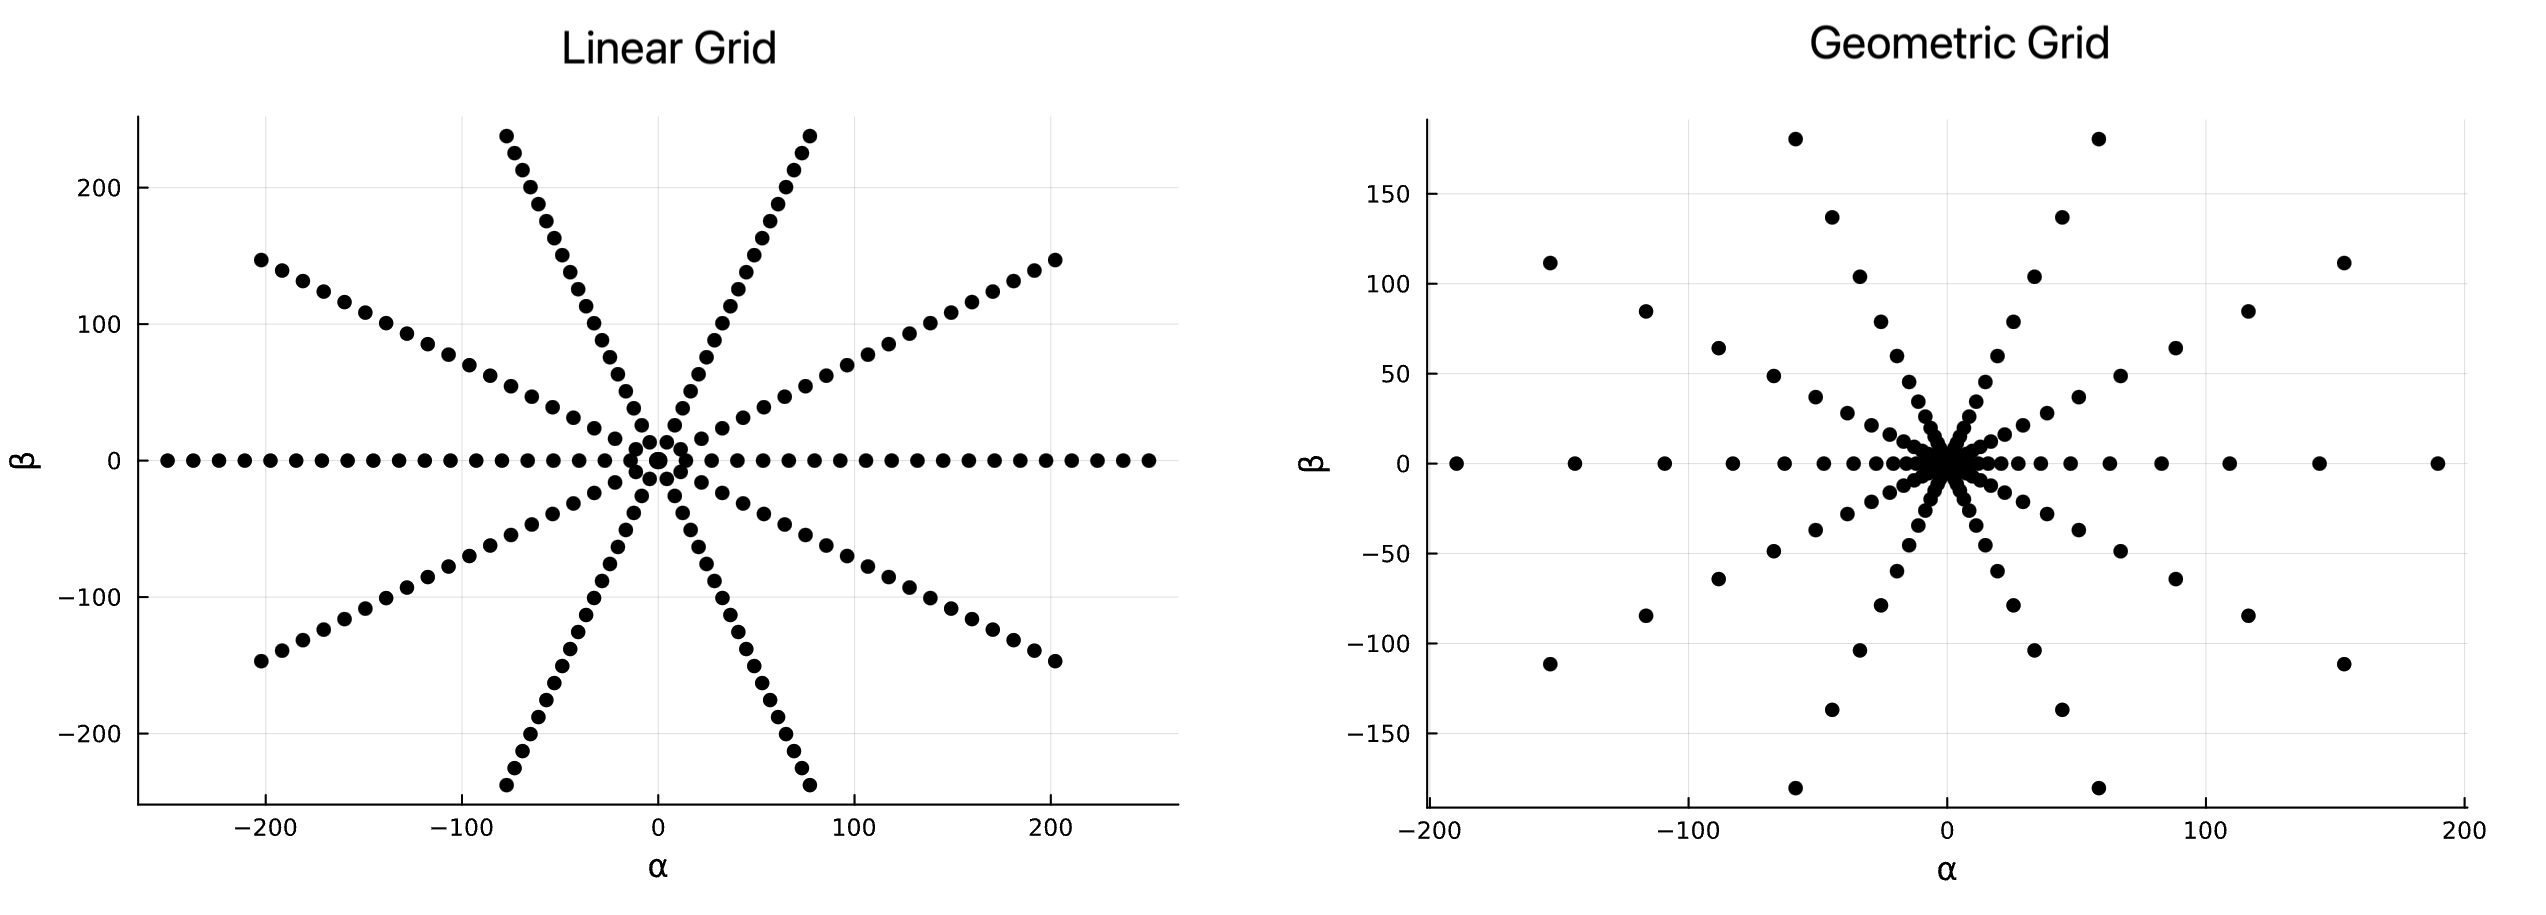
\includegraphics[width=0.98\linewidth]{figures/grid.png}
    \caption{Two grid models used in the binning method approach in calculating emissivity profiles. Every point corresponds to a geodesic hitting the disc and calculating the photon flux in this bin based on the value at the point of impact. $\alpha$ and $\beta$ are the impact parameters on the disc.}
    \label{grid}
\end{figure*}

\begin{figure}{l}{0.5\textwidth}
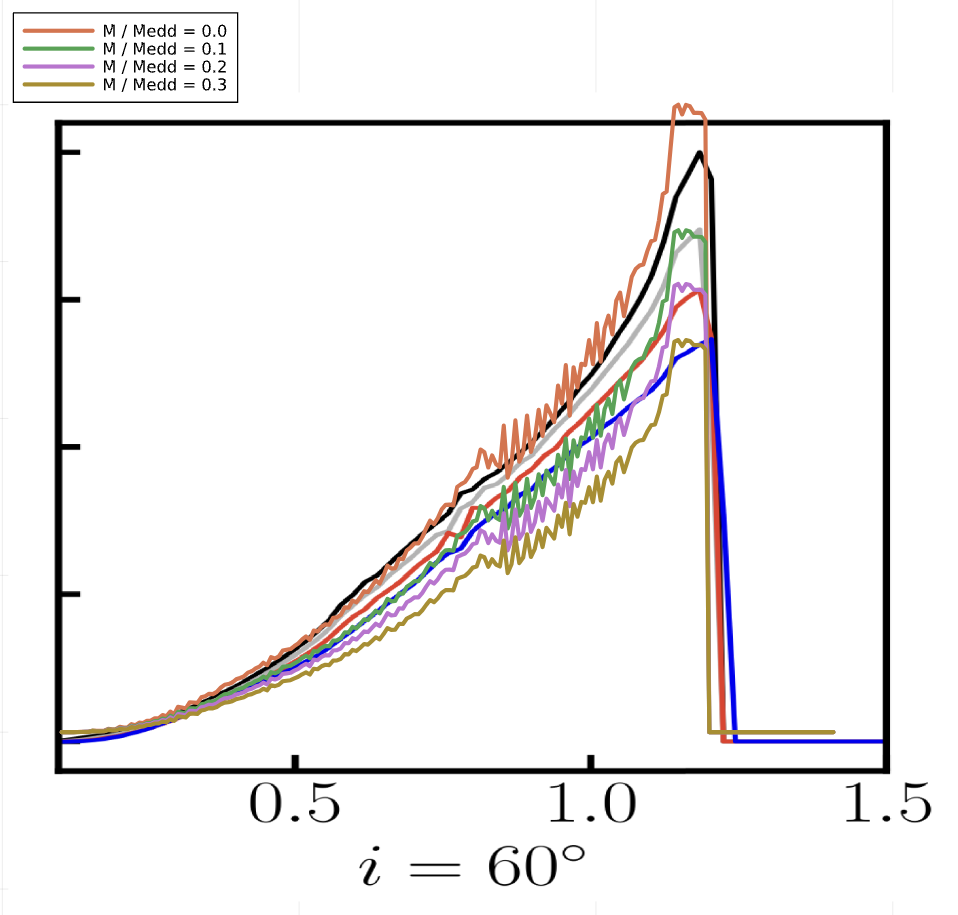
\includegraphics[width=\linewidth]{figures/lineargrid.png}
\caption{Replicated results from Figure \ref{taylorreynolds} for coronal height $h = 3 r_{g}$, inclination $\theta = 60^{\circ}$ and spin $a = 0.99$ overlaid over the results from \cite{taylor2018exploring} showing an improved, more consistent agreement in shapes when using the linear grid.}
\label{lineargrid}
\end{figure}

As clearly showed in the figure, the linear grid is more ``coarse'' with gaps visible at those important inner disc regions. This means, that if a geodesic hits that part of the disc, the flux is assumed to be uniform throughout the whole cell of the grid, possibly overweighting the strong flux contributions, since that is usually not the case. This becomes particularly pronounced at high inclinations and for thick discs, which is why the discrepancy appeared to intensify with both increasing inclination and disc height. As the disc gets thicker, there is more variation in the lines of constant redshift, so the error of the binning method which assumes a uniform flux becomes more pronounced. On the other hand, the ``finer'' grid provided by the geometric approach ensures the correct weighting of the flux since the geodesics concentrate around the inner part of the disc, making sure that this important region is handled correctly as it is more sensitive to the redshift lines variations. Overweighting the flux from the inner disc regions typically results in pointier line profiles, as seen in Reference \cite{taylor2018exploring}. 

To verify this hypothesis, the $\theta = 60^{\circ}$ inclination case from Figure \ref{taylorreynolds} was recreated (Figure \ref{lineargrid}) using the linear grid instead of the geometric one. As expected, the line profiles became pointier and agreed more with the results reported in the literature, suggesting the Authors did in fact overweight the flux contributions from the inner parts of the disc. A more appropriate method would involve the implementation of a linear grid or, even better, the transfer functions which have yielded us such reliable results so far.

% Johannsen self-consistently heights
After proving the importance of black hole geometry on shapes of the iron line profiles, the advancement of the self-consistent implementation of the Johannsen metric became an exciting prospect. For the first time not only was this metric modelled utilising a self-consistent calculation of the illumination pattern due to an isotropic lamp post corona, but it was also possible to simultaneously test the effects of varying multiple deviation parameters -- $\alpha_{13}$ and $\epsilon_{3}$.

For the only non-zero deformation parameter $\alpha_{13} = -0.35$ and a rapidly rotating black hole viewed at $\theta = 70^{\circ}$, Figure \ref{johannsen_selfconsistent} shows that the Johannsen metric follows the aforementioned trend of the impact of geometry increasing as the coronal height is decreased. Interestingly, for the corona located at $h = 15 r_{g}$ and $h = 10 r_{g}$ the line profile peak is shifted towards lower energies as the disc thickness decreases – the opposite of how the height influenced shapes in the Kerr metric (Figure \ref{taylorreynolds}). Whilst the effect was observed to become more prominent when comparing these two heights, for the lowest height $h = 5 r_{g}$ the energy shift was opposite and appeared to increase for thinner discs. The value of maximum flux reached appeared to increase as coronal height was decreased. This is attributed to more light being gravitationally focused by the black hole causing more photon paths to get bent in the strong gravitational field and hit the disc.

Results presented in Figure \ref{johannsen_deformation} are difficult to compare against literature as it is a novel approach where multiple deviation parameters in the Johannsen metric were varied and the iron line profiles calculated based on an irradiation pattern calculated utilising a self-consistent model of corona illuminating the disc.
Interestingly, increasing the value of the $\alpha_{13}$ parameter was expected to increase the observed flux value based on the previous results. This effect was not observed and increasing the deviation parameter did not follow the anticipated trend in the specific case investigated. Ideally, this should be investigated further -- as mentioned, rapidly rotating black holes are important from the observational standpoint and high inclination cases introduce interesting challenges to the numerical methods. The deviation from the expected trend could be possibly explained by the extreme regions of parameter space introduced in this scenario or potentially not appropriately handling the disc shadowing. For a quantitive conclusion, more detailed tests should be performed focusing on self-consistently calculated iron line profiles for rapidly rotating black holes viewed at high inclinations, although this can be extremely challenging.


% degeneracies
It was found in the literature that iron line profiles of Kerr-like objects are correlated with profiles of Kerr black holes if the parameters of spin and deformation parameters are chosen such that the innermost stable circular orbit coincides in both cases. For slowly or moderately spinning black holes with non-zero deviation parameters the profiles are almost impossible to differentiate, although for rapidly rotating black holes the same trend is not observed and if the deviation is high enough, the difference between the two objects is rather pronounced as outlined by \cite{johannsen2014x} and as further shown in this work in Figure \ref{johannsen_degeneracy}. For both cases in each plot, the parameters are such that the ISCO location coincides.

The mentioned reference models this phenomenon using the power law, arguing that the emissivity index is a function of the accretion disc radius and reaches higher values near the ISCO, which allows the iron lines to differ even for small values of the deformation parameters since the parts of the disc in closer vicinity of a black hole are most susceptible to strong relativistic effects whilst contributing more to the total observed flux, therefore making the deviations more meaningful in this region. \cite{psaltis2011ray} further studied the iron lines in the non-Kerr metrics and justified this broken correlation between spin and deformation parameters as the disc extending closer to the event horizon, where any deviation from the Kerr metric becomes most apparent.

Despite Reference \cite{johannsen2014x} investigating the degenerate iron line profiles using a model utilising a broken power law and this work implementing a point source lamp post corona, the two works remained consistent. Both showed the largest difference when comparing a Kerr black hole with spin $a = 0.95$ and zero deformation parameter $\alpha_{13}$ with a Kerr-like one with $a = 0.85$ and $\alpha_{13} = -1.07115$, whilst providing a good match between $a = 0.95$,  $\alpha_{22} = 0$ and $a = 0.85$, $\alpha_{13} = 0.97902$ and showing a small difference again for the $a = 0.85$ and $\alpha_{13} = -1.07115$ as the deformation parameter is increased. 

% corona discussion  -- extended corona
In the discourse about coronal models, there are a few things to keep in mind. One of them is how the X-ray source is shaped. Despite the lamp post model correctly predicting the emissivity steepness at small radii and being supported by direct measurements \cite{wilkins2012understanding}, the source corona most is likely extended in geometry \cite{wilkins2015driving}. Furthermore, observations of Seyfert galaxy Markarian 335 performed over variable length timescales between the years 2006 and 2013 showed that changes in the geometry of the corona and its energetics cause variability in the X-ray emission \cite{wilkins2015driving}. Long term, when considering the high flux emission the corona was observed to expand over the inner regions of the accretion disc, contracting in the intermediate and low-flux activity periods. Later observations divulged the source becoming extended vertically, implying an upward motion of the particles. Intrinsically, considering behaviour of the X-ray source is expected to affirm the mechanism responsible for powering energetic AGNs.

% corona discussion -- heights
Secondly, since the height of the corona impacts the profile significantly, it is important to choose the correct value for $h$. In fact, according to Reference \cite{fabian2014determination}, the broad features in the iron line profiles are observed if given rise to by a radiation source located below $h=10$. An idea of compact corona present in the vicinity of the black hole is further supported by spectral-timing and reverbation studies \cite{cackett2014modelling}; \cite{kara2013discovery}; \cite{uttley2014x}). A more detailed overview of coronal modelling can be found in \cite{dauser2016relativistic}.

Fit to data would be a useful test of this framework, making use of the archive data (including XMM-Newton and NuSTAR), and by comparing our model with existing, less sophisticated, models in the NASA XSPEC fitting package. 
When considering fitting of the emissivity profile, \cite{wilkins2015driving} outline a reliable method, although it is pointed out that for decomposition of the reflection spectrum, a good signal to noise detection in the iron line is necessary. Additionally, if the evolution of the corona is of interest, due to the flux variability, the long exposure observations are not possible without assuming the profile form in advance. Therefore, measurements from long observations and theoretical models are both considered and then the model is fitted to outline the spectrum influenced by the relativistic effects, forming an emissivity profile. This further shows the need for numerical modelling when considering profiles from black holes as it is an essential tool required for analysis. 
ATHENA mission could provide useful data where this approach could be implemented for modelling the profile form and tracing the relativistic effects.


\section{Conclusions}

Black holes provide an extremely interesting test of physics in extreme environments due to the strong gravitational force they are sources of. Despite being characterised by only three parameters -- mass ($M$), spin ($a$), and charge ($Q$) they stand behind some of the most exciting phenomena in modern astrophysics. X-ray radiation emitted from the accretion discs gives rise to spectra, amongst which the most prominent is the iron K$\alpha$ line. This element of the emissivity profile is particularly susceptible to deformation due to strong relativistic effects and serves as an excellent probe of the black hole geometry and its properties.

In this work, a novel photon integration code {\tt Gradus.jl} was utilised to create iron line profiles from black hole accretion discs to enable the study of general relativity and its effects. Two primary methods for iron line modelling were outlined and demonstrated and the differences between the two were discussed in depth. While the emissivity profile can be approximately described by the power law approximation, implementing a self-consistent model of a point source corona and therefore calculating the irradiation pattern of the disc accounts for the important effects of the black hole geometry on the observed spectrum. Additionally, it accounts for the steepness of the profile at small radii, which cannot be explained when considering the power law calculations. 

The intensity as a function of radius following a power law is dependent on the emissivity index which dictates the power of the profile. In self-consistent calculation, this is in turn dependent on the ratio of emitted to observed energy to the power of the photon index. The effects of varying this parameter followed the expected trend, becoming steeper at small radii as the value was increased. The influence of the coronal height on the emissivity profile was investigated to verify the correctness of the model and showed good consistency with the literature. Discrepancies were observed for low coronal heights in rapidly rotating black holes with spins $a = 0.99$ which increased with the inclination angle. Despite providing a possible solution to the problem and its proof it is hard to claim with certainty without the code used in the literature being publicly available. This proves not only the need for open-source access to the numerical simulations but also highlights the importance of multiple independent models needed to completely verify any new results. However, this solution is promising and alongside the rest of the state-of-the-art study presented in this work is intended to be written up as an article with more in-depth analysis after requesting the numerical simulation code used in Reference \cite{taylor2018exploring}.

As the height of the corona is increased, photon flux incident on the disc is focused on its innermost part with lower irradiation of the outer parts of the disc. The importance of the disc thickness was also discussed as it can lead to observation of an interesting phenomenon -- the disc shadowing, where the inner parts of the disc shield its outer parts from the photons emitted by the corona. However, this effect was observed to become less prominent for rapidly rotating black holes, due to the disc becoming more flat for the same values of Eddington ratio.

This rigorously tested numerical framework was then utilised to provide a more detailed investigation of cases noted as most interesting in the literature, focusing on rapidly rotating black holes observed at high inclination angles, due to their appeal for difficult to construct mathematical method as well as their observational applications.

High values of spin which contribute to the ISCO moving closer to the central black hole were found to increase the effects of the strong gravitational field on the line profile, although this effect is decreased by the increasing radiative efficiency which in turn makes the disc thinner and causes the differences between the disc heights to lessen compared to an infinitely thin disc model. The differences in line profiles on discs with different heights due to the $\alpha_{13}$ deformation parameter were observed to increase up to a rapidly rotating $a = 0.9$ case and then become less prominent for a maximally rotating black hole with spin $a = 0.998$. The self-obscuration of the disc was found to give rise to peaky feature in the iron line profiles, particularly for thicker discs viewed at high inclinations which then dissipated again as the disc flattened due to increased spin. No such features were observed in the self-consistently calculated profiles, implying dependency on the method and geometry. 

The Johannsen metric was discussed extensively and the impact of the introduced parameters describing deviation from the Kerr space-time was investigated. Typically, the $\alpha_{13}$ deformation parameter did not impact the profiles of non-rotating Schwarzschild black holes, but its effect on the profile was more obvious for rotating cases. Typically, increasing the value of the parameter $\alpha_{13}$ resulted in increased maximum flux whilst not following any clear trend when considering different disc heights. An exception occurred for a specific case of a rapidly rotating black hole with spin $a = 0.9$ and the coronal height $h = 6 r_{g}$ viewed by a distant observer at an inclination angle $\theta = 70^{\circ}$, where the impact of the deviation parameter did not follow a specific trend. Possible reasons for this were discussed, although more tests should be carried out to reach a viable conclusion.
A difference was observed when comparing the Johannsen metric modelled by approximation with the power law with the self-consistent method resulting in higher discrepancies in the maximum flux reached by discs of different thicknesses if the deformation parameter was higher. Most noticeable differences were observed for low-placed corona where the effects of geometry became most prominent. The line profiles appeared to shift the peak flux towards lower energies as the coronal height was increased and the shape of the line itself changed significantly depending on $h$. Overall, the maximum flux observed appeared to follow the trend of increasing with the corona located lower on the black hole rotation axis. For the first time, the effects of varying multiple deformation parameters were modelled self-consistently, illustrating the relationships between parameters. 

Finally, the interesting phenomenon of degenerate iron lines was tested utilising the coronal irradiation of the disc as opposed to the power law approximation. Cases of Kerr and Kerr-like black holes where the location of the innermost stable circular orbit coincides for different values of spin and a non-zero deviation parameter provide a possibility of degeneracy in the profiles at low and intermediate spins, although proved to be different for rapidly rotating black holes, provided the deviation is large enough. It would be interesting to see more work done concerning self-consistent variations of multiple deviation parameters, both regarding the possibility of degeneracies and their specific impact on the iron line profiles. Additionally, the self-consistent model ought to be studied in more depth, and whether the coronal height and the photon index contribute to degeneracy in iron line profiles.

\section*{Acknowledgements}

Thanks to various funding bodies and grants.

\section*{Data Availability}
 
The inclusion of a Data Availability Statement is a requirement for articles published in MNRAS. Data Availability Statements provide a standardised format for readers to understand the availability of data underlying the research results described in the article. The statement may refer to original data generated in the course of the study or to third-party data analysed in the article. The statement should describe and provide means of access, where possible, by linking to the data or providing the required accession numbers for the relevant databases or DOIs.

\bibliographystyle{mnras}
\bibliography{line-profiles}

\bsp
\label{lastpage}
\end{document}
